%stylefile for "Progress in Particle and Nuclear Physics" from 20. March 2003
\documentclass[twoside,12pt]{article}
\usepackage{graphicx}
\usepackage{lineno}
\bibliographystyle{elsarticle-num}
\def\Journal#1#2#3#4{{#1} {#2} (#4) #3 }
\def\NCA{{\em Nuovo Cimento} A}
\def\PHYS{{\em Physica}}
\def\NPA{{\em Nucl. Phys.} A}
\def\MATH{{\em J. Math. Phys.}}
\def\PRO{{\em Prog. Theor. Phys.}}
\def\NPB{{\em Nucl. Phys.} B}
\def\PLA{{\em Phys. Lett.} A}
\def\PLB{{\em Phys. Lett.} B}
\def\PLD{{\em Phys. Lett.} D}
\def\PL{{\em Phys. Lett.}}
\def\PRL{\em Phys. Rev. Lett.}
\def\PREV{\em Phys. Rev.}
\def\PREP{\em Phys. Rep.}
\def\PRA{{\em Phys. Rev.} A}
\def\PRD{{\em Phys. Rev.} D}
\def\PRC{{\em Phys. Rev.} C}
\def\PRB{{\em Phys. Rev.} B}
\def\ZPC{{\em Z. Phys.} C}
\def\ZPA{{\em Z. Phys.} A}
\def\ANNP{\em Ann. Phys. (N.Y.)}
\def\RMP{{\em Rev. Mod. Phys.}}
\def\CHEM{{\em J. Chem. Phys.}}
\def\INT{{\em Int. J. Mod. Phys.} E}
\def\r{\vec r}
\def\R{\vec R}
\def\p{\vec p}
\def\P{\vec P}
\def\q{\vec q}
\def\ss{\mbox{\boldmath $\sigma$}}
\newcommand{\be}{\begin{equation}}
\newcommand{\ee}{\end{equation}}
\newcommand{\bea}{\begin{eqnarray}}
\newcommand{\eea}{\end{eqnarray}}
\newcommand{\nn}{\nonumber}
\newcommand{\pT}{\mbox{$p_{\mathrm{T}}$}}
\newcommand{\vtwo}{\mbox{$v_2$}}
\newcommand{\energy}{\mbox{$\sqrt{s_{\mathrm{NN}}}$}}

\newcommand{\dd}{\mbox{$\mathrm{d}$}}
%\newcommand{\pp}{\mbox{$pp$}}
\newcommand{\AuAu}{\mbox{Au+Au}}
\newcommand{\PbPb}{\mbox{Pb+Pb}}%\mathrm{Pb}-\mathrm{Pb}$}}
\newcommand{\Ncoll}{\mbox{$N_{\mathrm{coll}}$}}
\newcommand{\Ncollcent}{\mbox{$N_{\mathrm{coll}}^{\mathrm{cent}}$}}
\newcommand{\Ncollperiph}{\mbox{$N_{\mathrm{coll}}^{\SixtyToEighty}$}}
\newcommand{\Rcollcent}{\mbox{$R_{\mathrm{coll}}$}}
\newcommand{\Npart}{\mbox{$N_{\mathrm{part}}$}}
\newcommand{\TAAb}{\mbox{$T_{\mathrm{AA}}(b)$}}
\newcommand{\TAA}{\mbox{$T_{\mathrm{AA}}$}}
\newcommand{\RAA}{\mbox{$R_{\mathrm{AA}}$}}
\newcommand{\Rcp}{\mbox{$R_{\rm CP}$}}
\newcommand{\delRcp}{\mbox{$\delta R_{\rm CP}^{\mathrm{sys}}$}}
\newcommand{\RTwo}{\mbox{$R= 0.2$}}
\newcommand{\RThree}{\mbox{$R = 0.3$}}
\newcommand{\RFour}{\mbox{$R = 0.4$}}
\newcommand{\RFive}{\mbox{$R = 0.5$}}
\newcommand{\RcpRatio}{\mbox{$R_{\mathrm{CP}}^{R}/R_{\mathrm{CP}}^{\,0.2}$}}
\newcommand{\kt}{\mbox{$k_{t}$}}
\newcommand{\antikt}{\mbox{anti-\kt}}
\newcommand{\sumet}{\mbox{$\Sigma E_{\mathrm{T}}$}}
\newcommand{\Nevt}{\mbox{$N_{\mathrm{evt}}$}}
\newcommand{\sqrts}{\mbox{$\sqrt{s_{\mathrm{NN}}}$}}
\newcommand{\vtwo}{\mbox{$v_2$}}
\newcommand{\vtjet}{\mbox{$v_2^{\mathrm{jet}}$}}
\newcommand{\Dphi}{\mbox{$\Delta \phi$}}
\newcommand{\pTjet}{\mbox{$p_{{\mathrm{T}}}$}}

\newcommand{\text}{\mbox}
\providecommand{\rd}{\mathrm{d}}
\newcommand {\lum}    {\ensuremath{150\,\mu\mathrm{b}^{-1}}}
\newcommand {\roots}    {\ensuremath{\sqrt{s}}}
\newcommand {\rootsNN}  {\ensuremath{\sqrt{s_{_{NN}}}}}
\newcommand {\sqrtsnn}  {\ensuremath{\sqrt{s_{_{NN}}}}}
\newcommand {\dndy}     {\ensuremath{{\rd}N/{\rd}y}}
\newcommand {\dnchdy}   {\ensuremath{{\rd}N_{\text{ch}}/{\rd}y}}
\newcommand {\dndeta}   {\ensuremath{{\rd}N/{\rd}\eta}}
\newcommand {\dnchdeta} {\ensuremath{{\rd}N_{\text{ch}}/{\rd}\eta}}
\newcommand {\dndpt}    {\ensuremath{{\rd}N/{\rd}\pt}}
\newcommand {\dnchdpt}  {\ensuremath{{\rd}N_{\text{ch}}/{\rd}\pt}}
\newcommand {\deta}     {\ensuremath{\Delta\eta}}
\newcommand {\dphi}     {\ensuremath{\Delta\phi_{1,2}}}
\newcommand {\AJ}       {\ensuremath{A_J}}
\newcommand {\npart}    {\ensuremath{N_{\text{part}}}}
\newcommand {\ncoll}    {\ensuremath{N_{\text{coll}}}}

\newcommand {\pp}    {\mbox{p+p}}
\newcommand {\ak} {anti-$k_\text{T}$}
\newcommand {\pt} {\ensuremath{p_{\rm{T}}}}
\newcommand {\ptlead} {\ensuremath{p_{\rm{T},1}}}
\newcommand {\ptsub} {\ensuremath{p_{\rm{T},2}}}
\newcommand {\ptrat} {\ensuremath{\ptsub/\ptlead}}

\newcommand {\tev}       {\ensuremath{\,\mathrm{TeV}}}
\newcommand {\TeV}       {\ensuremath{\,\mathrm{TeV}}}
\newcommand {\GeV}       {\ensuremath{\,\mathrm{GeV}}}
\newcommand {\GeVc}      {\ensuremath{\,\mathrm{GeV/c}}}
\newcommand{\stat}{\ensuremath{\,\text{(stat.)}}}
\newcommand{\syst}{\ensuremath{\,\text{(syst.)}}}

\newcommand{\m}{\ensuremath{\,\text{m}}}
\providecommand{\mb}{\mbox{\,\mathrm{mb}}}
\providecommand{\nb}{\mbox{\,\mathrm{mb}}}
\newcommand {\naive}    {na\"{\i}ve}
\newcommand{\PHOJET} {\textsc{phojet}}
\newcommand{\HYDJET}{\textsc{hydjet}}
\newcommand{\PYTHYD}{\textsc{PYTHIA+HYDJET}}
\newcommand{\PYTHIA}{\textsc{PYTHIA}}
\newcommand{\mboxwidth}{\textwidth}
\newcommand {\photonjet}{photon+jet}
\newcommand{\Pgpz}{\ensuremath{\pi^0}}
\newcommand{\Pgh}{\ensuremath{\eta}}
\newcommand{\Pgg}{\ensuremath{\gamma}}
\newcommand{\cPqb}{\ensuremath{b}}

\newcommand {\ptg}    {\ensuremath{p_{\mathrm{T}}^{\Pgg}}}
\newcommand {\ptj}    {\ensuremath{p_{\mathrm{T}}^{\text{Jet}}}}
\newcommand {\phig}    {\ensuremath{\phi^\Pgg}}
\newcommand {\phij}    {\ensuremath{\phi^\mathrm{Jet}}}

\providecommand{\ptjet}{\ptj}
\providecommand{\ptgamma}{\ptg}
\providecommand{\ptphoton}{\ptg}
\providecommand{\rjg}{\ensuremath{R_{J\Pgg}}}
\providecommand{\xjg}{\ensuremath{x_{J\Pgg}}}
\providecommand{\sjg}{\ensuremath{\sigma(\Delta\phi_{J\Pgg})}}
\providecommand{\ptg}{\ensuremath{p_{\mathrm{T},\Pgg}}}
\providecommand{\dphijg}{\ensuremath{\Delta\phi_{J\Pgg}}}
\providecommand{\avexjg}{\ensuremath{\langle x_{J\Pgg}\rangle}}
\providecommand{\sigeta}{\ensuremath{\sigma_{\eta\eta}}}

\providecommand {\mubinv}{\ensuremath{\mathrm{\mu b^{-1}}}}
\providecommand{\PHOJET} {\textsc{phojet}}
\newcommand {\dNdxsi} {\ensuremath{dN_{\mathrm{track}}/d\xi}}

\newcommand{\Jpsi}{\rm J/$\psi$}
\newcommand{\jpsi}{\rm J/$\psi$}
\newcommand{\JPsi}{\rm J/$\psi$}
\newcommand{\psip}{$\psi^\prime$}
\newcommand{\jpsiDY}{\rm J/$\psi$\,/\,DY}
\newcommand{\chic}{$\chi_{\rm c}$}
\newcommand{\ezdc}{$E_{\rm ZDC}$}
\newcommand {\cc}        {\ensuremath{{\mathrm c}\bar{{\mathrm c}}}}
\newcommand{\lumi}{\ensuremath{\mathcal{L}}}
\newcommand{\taa}        {\ensuremath{T_\mathrm{AA}}}
\newcommand {\Raa}       {\ensuremath{R_\mathrm{AA}}}
\newcommand {\y}         {\ensuremath{y}}
\newcommand {\meanptsq}  {\ensuremath{\langle p_{\mathrm{\textsc{t}}}^{2} \rangle}}
\newcommand {\nucnuc}    {\ensuremath{\mathrm{A\mbox{-}A}}}
\newcommand {\pPb}       {\ensuremath{\mathrm{p\mbox{-}Pb}}}
\newcommand {\vpt}       {\mbox{$v_2(p_{\rm T})$ }}
\newcommand{\PgU}{\ensuremath{\Upsilon}}
\newcommand{\PgUa}{\ensuremath{\Upsilon\mathrm{(1S)}}}
\newcommand{\PgUb}{\ensuremath{\Upsilon\mathrm{(2S)}}}
\newcommand{\PgUc}{\ensuremath{\Upsilon\mathrm{(3S)}}}
\newcommand{\PgUd}{\ensuremath{\Upsilon\mathrm{(3S)}}}
\newcommand{\PgUn}{\ensuremath{\Upsilon\text{(nS)}}}
\newcommand{\nbinv} {\mbox{\ensuremath{\,\text{nb}^{\text{$-$1}}}}}
\providecommand{\Pap}{\ensuremath{\mathrm{\overline{p}}}}
\providecommand{\Pp}{\ensuremath{\mathrm{{p}}}}



\topmargin-2.8cm
\oddsidemargin-1cm
\evensidemargin-1cm
\textwidth18.5cm
\textheight25.0cm
\begin{document}

\linenumbers

\title{ \vspace{1cm} Heavy-ion collisions at the LHC}
\author{G.\ Roland$^{1}$, K.\ \v{S}afa\v{r}\'{\i}k$^2$, P.\ Steinberg$^3$\\
\\
$^1$Massachusetts Institute of Technology, Cambridge, MA 02139, USA\\
$^2$CERN, European Organization for Nuclear Reasearch, Geneva, Switzerland\\
$^3$Brookhaven National Laboratory, Upton, NY 11973, USA\\
}
\maketitle
\begin{abstract} 
A new era in the study of high-energy nuclear collisions began when the 
CERN Large Hadron Collider (LHC) provided the first collisions of lead nuclei
in late 2010. In the first three years of operation the ALICE, ATLAS and CMS 
experiments each collected \PbPb\ data samples of more than 150\mubinv at 
$\rootsNN = 2.76$\TeV, exceeding the previously studied collision energies 
by more than an order of magnitude. These data have provided new insights into
the properties of QCD matter under extreme conditions, with extensive
measurements of soft particle production and newly accessible probes
of hard probes of the hot and dense medium. In this review, we provide
a comprehensive overview of the results obtained in heavy-ion collisions
at the LHC so far, with particular emphasis on the complementary nature
of the observations by the three experiments.
In particular, the combination of ALICE's strengths at hadron identification
the strengths of ATLAS and CMS to make precise measurements of high \pT
probes, and the resourceful measurements of collective flow by all of the
experiments have provided a rich and diverse dataset in only a few years.
While the basic paradigm established at RHIC -- that of a hot, dense medium that flows with a viscosity to
entropy ratio near the predicted lower bound, and which degrades the energy
of colored probes, such as jets and $J/\psi$ -- is confirmed at the LHC,
the new data suggest many new avenues for extracting its properties in detail.
\end{abstract}

\eject
\tableofcontents
\section{Introduction}
\label{secall:intro}
The first ideas about heavy-ion experiments at the Large Hadron Collider (LHC)~\cite{Evans:2008zzb} at CERN were formed in the early nineties (in the last century)~\cite{Jarlskog:1990dv}. Since the beginning of the LHC project, approved by CERN Council in 1994, the investigation of heavy-ion collisions was an integral part of the LHC physics programme. Built from 1998 to 2008 in the 27~km long (approximately) circular underground tunnel, exploited before by the Large Electron--Positron (LEP) collider, the LHC machine represents the highest-energy particle accelerator ever made. This very versatile collider is designed to reach centre-of-mass energies up to $\sqrt{s} = 14$~TeV for proton--proton (pp) collisions, and up to 1\,150~TeV using lead-ion beams, corresponding to $\sqrt{s_{\rm NN}} = 5.5$~TeV per colliding nucleon pair. These will entail the energy increase by a factor of seven for hadron collisions, and and more than 27 for heavy-ion collisions compared to predecessor colliders.
\subsection{Physics motivation}
\label{subsecall:motivation}
At very high temperatures and densities, hadronic matter is expected to undergo a phase transition into a qualitatively different state, where quark and gluon degrees of freedom are liberated. Such conditions were prevailing in the early Universe, a few microseconds after its formation. In heavy-ion collisions at ultra-relativistic energies, nuclear matter is heated and compressed reaching conditions well beyond the phase-transition point, and the same type of medium filling the very early Universe is thus momentarily re-created. At the highest available energies, at the LHC, far better conditions, than those at the other existing facilities, are achieved to study this new state of matter, called the Quark--Gluon Plasma (QGP). The nearly-vanishing baryon density, the highest available initial temperature and energy density, and the abundance of perturbatively-calculable hard Quantum Chromo-Dynamics (QCD) processes make heavy-ion collisions at the LHC particularly well-suited for precision studies of the QGP properties.

QCD, the well-established theory of strong interactions, predicts (cross-over) phase transitions in strongly interacting matter at high temperatures. A phase transition reflects breaking of a fundamental symmetry in the theory. Above the critical temperature, ordinary hadronic matter, where protons and neutrons are composed of quarks and gluons confined in a colour-neutral state, melts during the deconfinement phase transition. In the deconfined medium, quarks and gluons are not bound into hadrons anymore, however, the effective degrees of freedom of the QGP, formed at temperatures achieved with heavy-ion collisions, are rather complex. A second phase transition is connected with the generation of hadron masses as a consequence of the presence of a quark--antiquark condensate in the vacuum at low temperature. According to QCD, at high temperatures, the vacuum condensate is reduced, and the masses of quarks drop to their bare values during a chiral phase transition. Quantitative lattice QCD calculations~\cite{Borsanyi:2010bp} confirm that QCD matter undergoes a transition from a hadronic gas to a QGP at a temperature about 160~MeV, corresponding to an energy density of about 0.5~GeV/fm$^3$. At LHC conditions (small baryon density), the transition is a smooth cross-over spanning a temperature range of 20--30~MeV, which means that the precise value of the critical temperature depends on the observable used to locate it.

In a heavy-ion collision the energy deposited at the mid-rapidity is determined by the density of low-$x$ (Bjorken $x$, corresponds approximately to the fraction of nucleon longitudinal momentum carried by a parton) gluons confined in the colliding nuclei. The relevant values of $x$ at LHC energies are order of magnitude smaller than those at RHIC, i.e. on the $10^{-3}$ level and below. In such small-$x$ range, at low virtualities the perturbative gluon distribution reaches the saturation and gluons have to fuse, in order not to violate unitarity.  This marks the transition to the non-linear parton-evolution region, and the virtuality scale at which this transition happens is known as the saturation scale $Q_{\rm s}$. It increases (logarithmically) with the incident energy, and the mass of colliding nuclei (as nucleon radius), and  reaches the values $Q_{\rm s} \approx 3$--$4$~GeV$^2$ for Pb--Pb collisions at the LHC. During the collision of the two nuclei, these dense gluon fields are deconfined and create a primordial strongly-interacting medium, which rapidly expands and thermalizes. The thermalized QGP continues to cool down, mainly by the longitudinal expansion, until its temperature decreases below the critical temperature of the QCD phase transitions, and then it is converted into a gas of hadron resonances. At this moment the produced-particle composition is frozen, and the corresponding temperature is called the chemical freeze-out temperature ($T_{\rm ch}$), presumably being close to the critical temperature of the QCD phase transitions. Hadrons still continue to interact, however, as their relative energy is below the threshold for inelastic production, only their momentum spectra are modified. At a kinetic freeze-out, with corresponding kinetic freeze-out temperature ($T_{\rm kin}$), the medium is diluted that the final hadrons decouple, ceasing any interaction with the rest.

Prior to the start-up of the LHC heavy-ion programme, the nature of the QGP as an almost-perfect, inviscid liquid emerged from the experimental investigations at RHIC~\cite{Tribble:2007nsac}. The pressure created in the thermalized QGP phase is reflected in the large azimuthal asymmetry observed in the final-state particle production. The resistance of the medium  to the shape change implies a very low shear viscosity, or in dimensionless variable, a very low ratio of shear-viscosity to entropy-density in the QGP. Consequently, it evidences extremely short mean-free path inside the medium at this stage of the evolution (and the corresponding cross section approaching the unitarity limit) induced by a complex excitation modes in strongly-coupled QCD medium. This also implies the development of the collective transverse velocity field at this stage, which contributes to the plasma cooling. The smallness of the mean-free path with respect to the system size allows for the successful utilization of relativistic hydrodynamics in the description of the evolution of the thermalized QGP until hadronization.

Such an interpretation is further supported by the observation of the strong energy loss of partons traversing this strongly-coupled QCD medium, demonstrated at RHIC with large suppression of particle production at transverse momenta ($p_{\rm T}$) up to 20~GeV. Deduced from these measurements, the large amount of the energy loosed by hard partons due to the gluon bremsstrahlung and by elastic collisions is consistent with the low shear viscosity established from the collective-flow pattern of low-momentum hadrons. With the first LHC data, this basic picture is confirmed, observing the creation of deconfined matter at unprecedented values of temperatures, densities and volumes~\cite{Muller:2012zq}. The origin of this almost-perfect-fluid QGP behaviour  is the subject of further experimental study at the LHC. Among the interesting interrogations to answer are: if the predicted initial gluon saturation reduces also the low-$p_{\rm T}$ particle yields; and if the low shear viscosity is affected by the expected increase of the QGP temperature at an early stage. However, the most important impact of the more than order of magnitude increase of the collision energy is the much higher rates for hard probes, such as the jets, electro-weak particles, heavy flavours, and quarkonia. The high rates allow for precision studies of the QGP using the in-medium interactions of these probes, better controlled theoretically than the propagation of light partons. In addition, some observables, e.g. very high-energy jets, electro-weak bosons, and different $\Upsilon$ states, are accessible in heavy-ion collisions for the first time. A comprehensive compilation of theoretical predictions for the LHC heavy-ion programme was published in~\cite{Abreu:2007kv}.
 
The experimental results obtained using heavy-ion collisions during the first period of the LHC running are summarized in this article. It is divided into the sections according to various heavy-ion observables: Sec.~\ref{secks:eventchar} describes the principals of centrality selection and measurements of particle and energy densities; particle yields and spectra are discussed in Sec.~\ref{secks:spectra}; correlation studies are explicated in Sec.~\ref{secks:nonflow} for non-flow effects, and in Sec.~\ref{sec:ps:flow} for flow phenomena; Sec.~\ref{sect:pas:ew} deals with production of electro-weak particles; Sec.~\ref{jets_intro} is dedicated to jets and their quenching; and to heavy flavours two sections are devoted, Sec.~\ref{secks:heavy} to open heavy flavours, and Sec.~\ref{} to quarkonia. Summary and outlook are given in Sec.~\ref{secall:summary}.

\subsection{LHC heavy-ion running}
\label{subsecall:running}

\begin{figure}[!htb]
\begin{center}
\includegraphics[width=0.8\textwidth]{introduction_figs/LHC_chain.png}
\caption[]{Schematic view of LHC injector chain, showing the path of both protons and ions.}
\label{fig:pas:intro:lhc}
\end{center}
\end{figure}

Heavy ion running at the Large Hadron Collider had been planned long before the machine was built.
This was based on the interest in the physics at the CERN SPS, which was colliding light ions since
1986 and heavy ions since 1994, and as a natural extension to the already-planned program
at the Relativistic Heavy Ion Collider (RHIC).
The accelerator complex is shown in Figure~\ref{fig:pas:intro:lhc}.
Ions start their path to collisions at the ECR (electron cyclotron resonance) ion source,
which provides lead ions stripped to values around Pb$^{29+}$, which are passed through
a spectrometer to select Pb$^{29+}$ and accelerated in a linear accelerator to 4.2 MeV/n.
They are then stripped to around Pb$^{54+}$ by a 0.3 $\mu$m carbon foil and the
Pb$^{54+}$ are selected by a spectrometer to be fed into the CERN Low Energy Ion Ring (LEIR).
LEIR is used to transform a set of low intensity ion pulses from the LINAC into shorter
bunches with higher intensity.  This is done by filling the available phase space in
three dimensions.  After this, electron cooling is applied to shrink the beam to increase the
bunch density, and decelerate it into ``a stack sitting slightly inside the central orbit''.
At this point, seven pulses are captured, split into two bunches, and then accelerated to
72 MeV/n.
The bunches from LEIR are then sent to the CERN PS (Proton Synchrotron), accelerated to
5.9 GeV/n and stripped fully to Pb$^{82+}$ using a 0.8 mm aluminium foil.  These ions
are then sent to the SPS where they are acceleated to 177 GeV/n and injected into the LHC.

To date, there have been three heavy ion runs at the LHC.
The first run was in November/December 2010,
which provided 120 colliding bunches of lead ions in each ring, with a center of mass energy per nucleon
pair of $\energy =2.76$ TeV, a peak luminosity of $3 \times 10^{25} / \mathrm{cm}^2 s$ and an integrated luminosity
of 7 $\mu \mathrm{b}^{-1}$, corresponding to about 50 million minimum bias events.
The second run was in November/December 2011, which provided about 360 colliding bunches of lead ions per ring,
also at $\energy =2.76$ TeV, a peak luminosity of
about $5 \times 10^{26}  / \mathrm{cm}^2 s$ and an integrated luminosity of
about 150 $\mu \mathrm{b}^{-1}$, a factor of 20 increase over 2010.
The third run, in January/February 2013, provided proton-lead collisions
at $\energy=5.02$ TeV but these results are not discussed
in detail in this review.

\subsection{Detectors at the LHC}
\label{subsecall:detectors}

Three, out of the four principal LHC detectors, participate in the LHC heavy-ion programme. These are: ALICE (A Large Ion Collider Experiment), a dedicated heavy-ion detector designed to operate in the high particle density environment; and two general-purpose particle detectors, ATLAS (... Toroidal ... whatever) and the CMS (Compact Muon Spectrometer), optimized to high interaction rates and capable of precision measurements at very high transverse momenta. The fourth detector, the LHCb, was not taking data in Pb--Pb runs due to the occupancy limitation, however, it participated in the p--Pb run, and reported interesting results. 

\subsubsection{ALICE}

\begin{figure}
\begin{center}
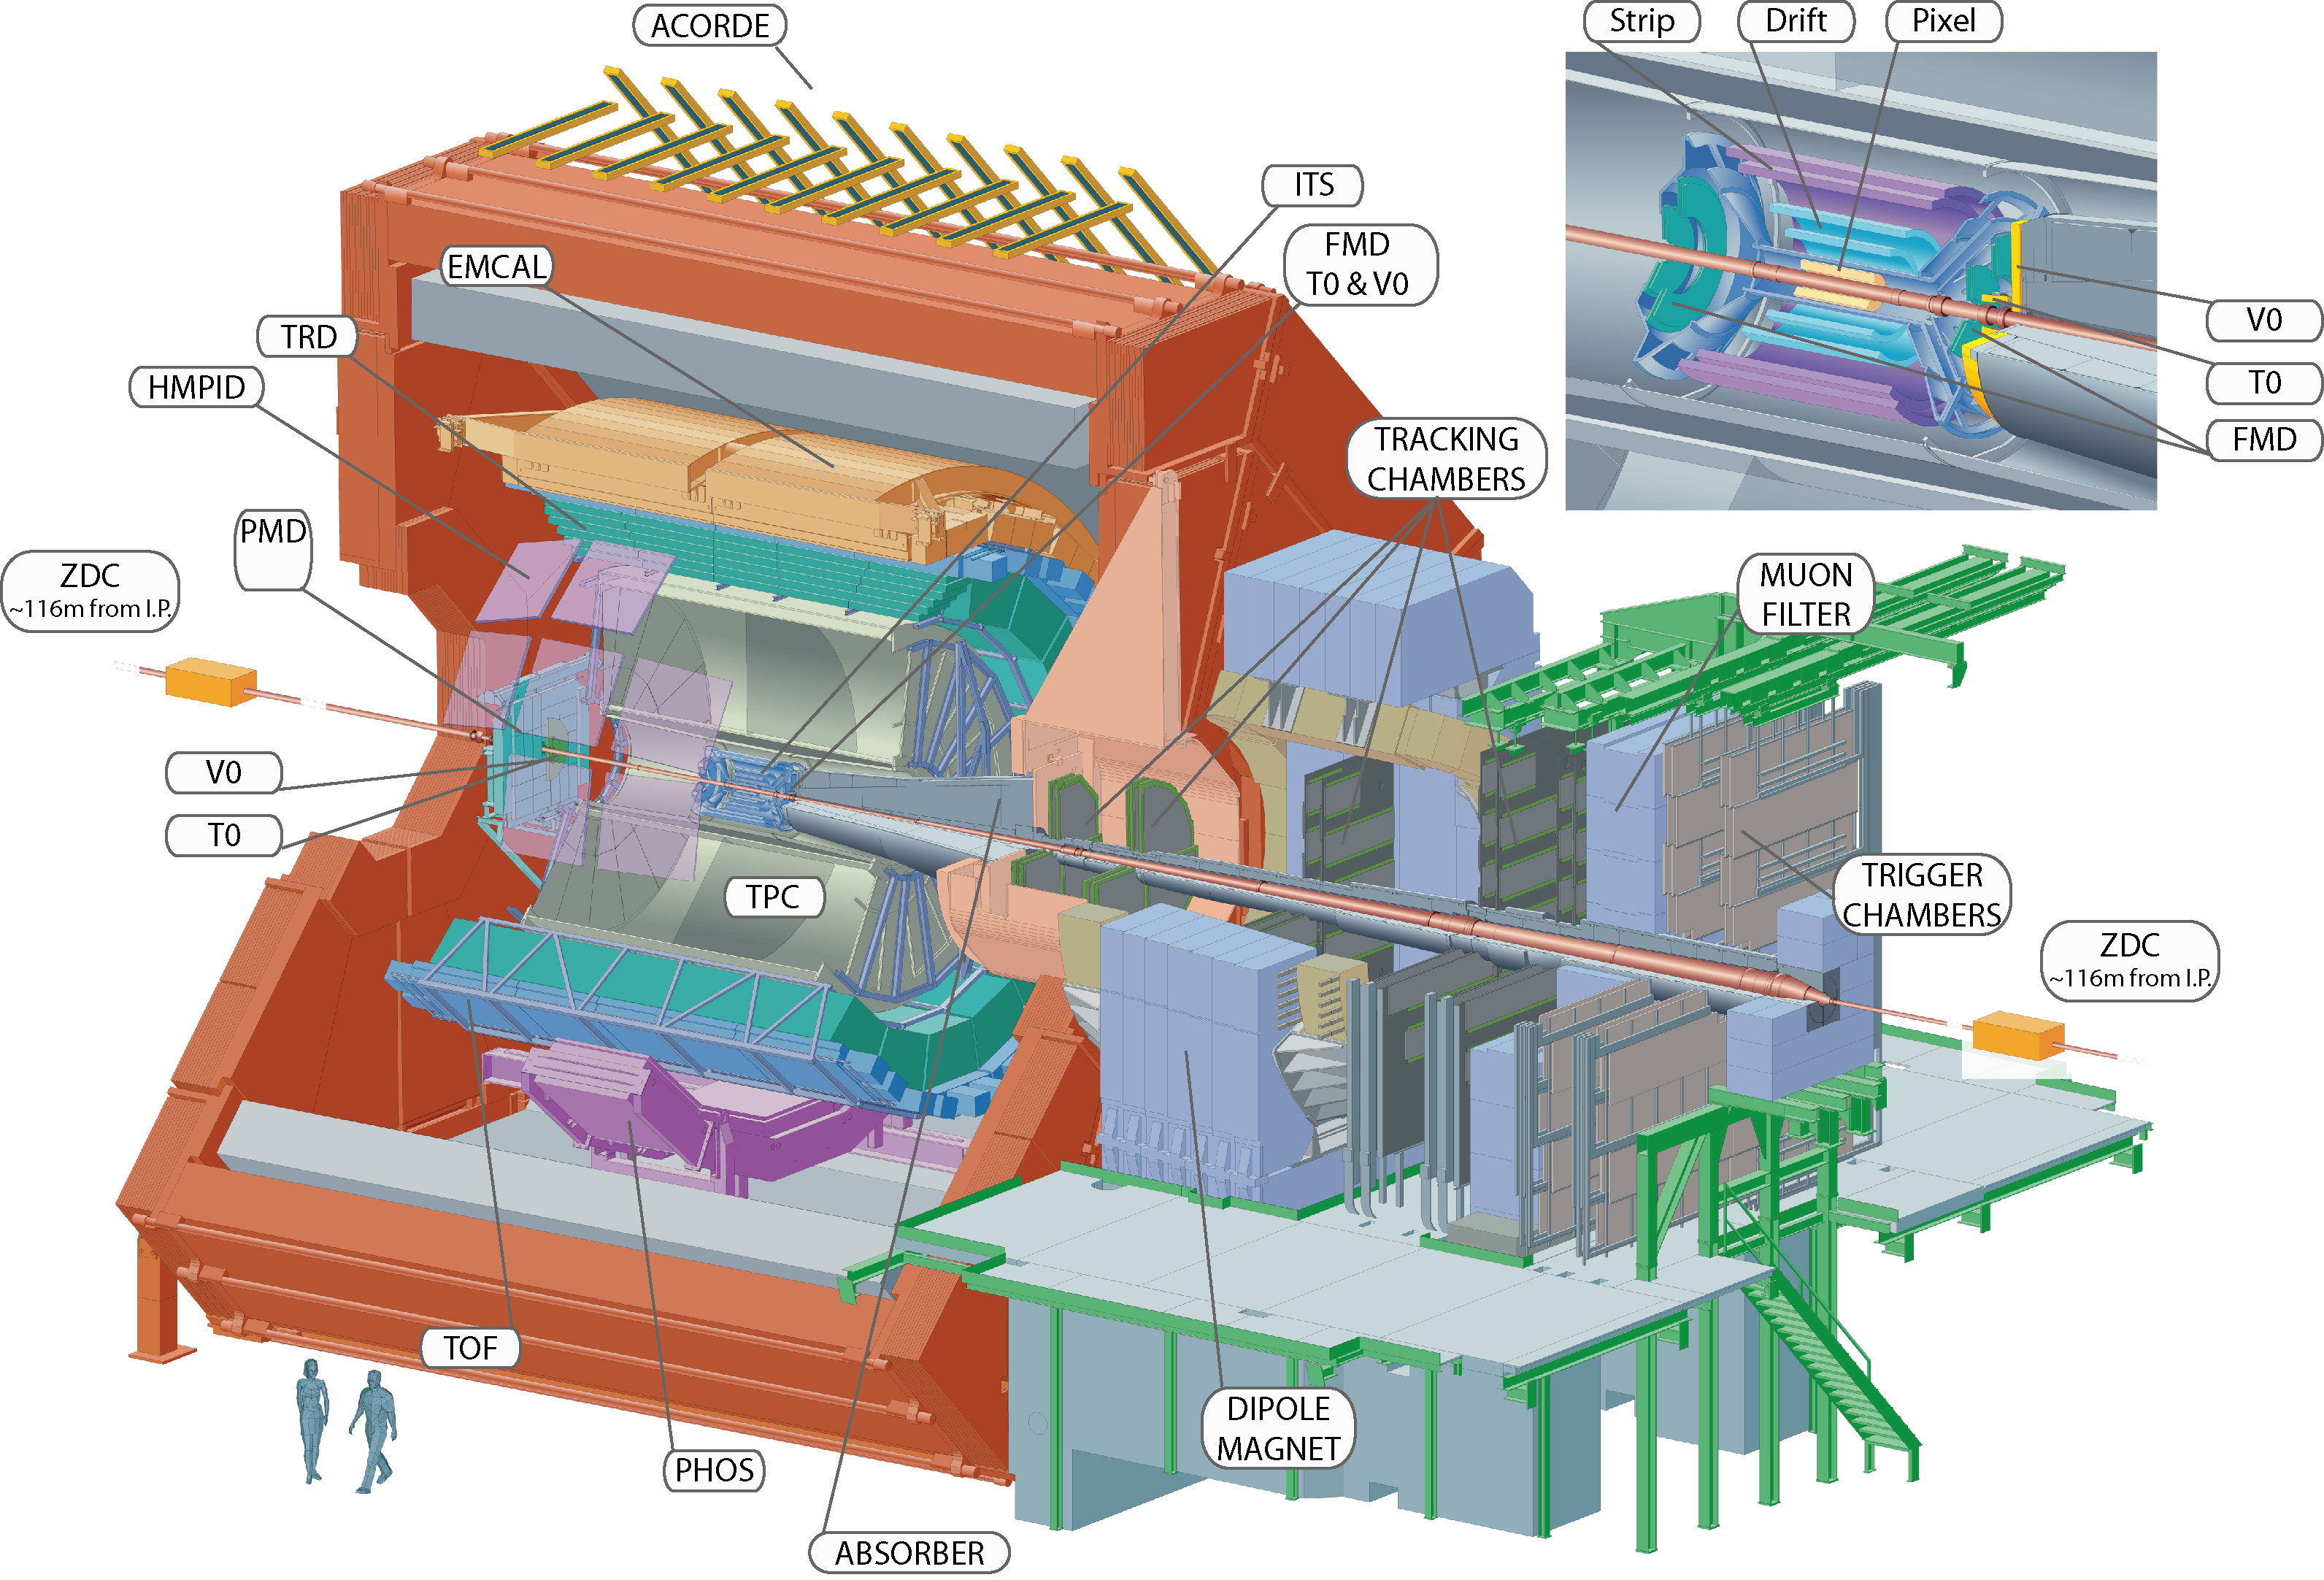
\includegraphics[height=0.49\textwidth]{introduction_figs/ALICEdet.png}
\caption{Schematic layout of the ALICE detector, indicating the main subsystems. The inset in top-right corner shows the innermost part in detail.}
\label{figks:ALICEdet}
\end{center}
\end{figure}


The ALICE detector~\cite{Aamodt:2008zz} is shown in Fig.~\ref{figks:ALICEdet}, and it has the following main parts: central barrel, muon arm, and forward detectors. The central barrel is housed in a large solenoid magnet providing the field of 0.5~T, with 12~m aperture and 12~m length, which was inherited from the L3 experiment running at the LEP collider. This part provides measurements of particles produced within about $\pm 45^\circ$ with respect to a plane perpendicular to the beam axis, corresponding to pseudorapidity coverage $|\eta| < 0.9$ ($\eta = - \ln \tan (\Theta/2)$, where $\Theta$ is the angle from the beam axis). The six-layer silicon Inner Tracking System (ITS), surrounding the beryllium vacuum beam pipe 6~cm in diameter, begins with pixel detectors at radii 4 and 8~cm, continues with silicon-drift detectors at 14 and 22~cm, and ends with double-sided strip detectors at 39 and 43~cm. The ITS measures the particle tracks with position precision of a few tens of microns. In addition, the four outer layers participate in the Particle Identification (PID) by determining the specific ionization energy loss (${\rm d}E/{\rm d}x$). The excellent spatial resolution of the innermost silicon pixel layers results in outstanding capabilities of primary and secondary vertex reconstruction.  The resolution in measuring the distance of closest approach to the primary vertex for tracks coming from secondary decays is for transverse momentum \pT of 1~GeV between 60--70~$\mu$m, allowing to detect weak decays of charm and beauty particles.
The main particle tracking device is the TPC (Time Projection Chamber), the largest such detector built to now. It has a cylindrical shape, more than 5~m along the beam axis, and 5~m in outer diameter. The TPC continues the tracking from the ITS at a radius of 88~cm and carries on till the end of its sensitive volume. The TPC volume, filled with neon-based gas mixture, is divided into two halves by a thin central high-voltage electrode providing an electrostatic field of about 0.4~kV/cm. Electrons created by ionization in the gas drift towards one of the end-plates equipped with multi-wire proportional chambers with cathode-pad readout. Altogether the TPC is read out with more than 600~thousands pads, which gives, taking into account the sampling along the drift direction, an effective granularity in the TPC volume of more than half a billion three-dimensional pixels. Consequently, this results in very efficient track-finding down to low transverse momenta, about 100~MeV, even at the highest particle densities in central lead--lead collisions at LHC energies. In addition, the ALICE TPC has an excellent resolution for the measurement of ${\rm d}E/{\rm d}x$, between 5 and 6\,\%, depending on particle density. 
The momentum dependencies of ${\rm d}E/{\rm d}x$ for different particles cross when approaching their minima for ionization energy losses. This makes particle identification using such method impossible in that momentum region. To distinguish particle species in this region, ALICE installed a Time-Of-Flight detector (TOF) at a radius of about 3.7~m from the beam axis. This detector determines the arrival time of charged particles with a precision better than 100~ps, exploiting multi-gap resistive plate chambers, an innovative technology developed specifically for ALICE. The TOF measurement is able to separate pions and kaons up to 2.2~GeV, K mesons and protons up to 3.5~GeV, and can be used for electron identification at lower momenta. To further increase the momentum reach for charged hadron identification, a smaller detector, the High-Momentum PID (HMPID), covering about 10\,\% of to the other central barrel detectors and using \v{C}erenkov ring-imaging technique, is placed at a distance of 1~m larger than that of TOF. To improve the electron identification ALICE uses a Transition Radiation Detector (TRD) situated between the TPC and TOF detectors. Particles traverse six radial drift chambers, each consisting of a transition radiator followed be a volume containing a xenon-based gas mixture, allowing the detection of X-ray photons in addition to charged tracks. The TRD drift chambers are read out with cathode-pad wire chambers. Electrons are separated from pions by discriminating on signal amplitude of last samples, where the electron transition radiation contributes. This detector is also used in the tracking system; an increase of the track length in magnetic field improves the momentum resolution at high transverse momenta (to about 5\,\% around 100~GeV). At low momenta, 0.1--1~GeV, the momentum resolution of ALICE tracking system is better than 1\,\%. The central barrel part of ALICE is completed with electromagnetic calorimeters. The larger one, EMCal, covers $120^\circ$ in azimuthal angle and in longitudinal direction a little less than the barrel detectors in front of it. It is used to trigger on jets and to improve the jet energy determination measured with tracking detectors. The much smaller Photon Spectrometer (PHOS) has significantly better energy resolution and granularity, and is dedicated to the isolation of a direct photon signal in heavy-ion collisions.

The ALICE detector can detect and trigger on muons in the forward region on one side of the central barrel using its muon arm, between $2^\circ$ and $9^\circ$ from the beam axis. A conical absorber begins at only 90~cm from the nominal interaction point, in order to suppress the background from decaying pions and kaons. Behind the absorber, the five tracking stations detect the filtered out muons. The first two stations are still inside the main solenoid magnet; the third one is in the middle of the ancillary dipole magnet with 3~Tm of field integral used for muon momentum analysis; the remaining two measure deflected muon tracks behind the dipole. Each tracking station consists of two planes of multi-wire chambers with cathode-pad readout, giving a coordinate precision of about 100~$\mu$m in the bending plane, thus giving a mass resolution of 1\,\% at the $\Upsilon$ mass, needed for the separation of different $\Upsilon$ states. Behind the last muon tracking station a second absorber shields the muon trigger detectors from remaining background. The full length of the muon arm, from the interaction point to the end of the trigger system, is about 20~m. Two trigger planes of Resistive Plane Chambers (RPC) detect the position and direction of penetrating muons. Using this information the muon trigger electronics select events having muons with transverse momentum above a predetermined threshold.

On the side opposite to the muon arm the Photon Multiplicity Detector (PMD) measures the yield of $\pi^0$ mesons by counting the number of photons. The Forward Multiplicity Detector (FMD), with silicon strip planes on both sides of the interaction region, determines the density of charged particles emitted at pseudorapidities $-3.4 < \eta -1.7$ and $1.7 < \eta < 5$. Scintallator tile arrays (called VZERO), covering similar acceptance to the FMD, are used to trigger on LHC collisions, in heavy-ion collisions also selecting different centrality classes with corresponding thresholds. Small quartz counters on both sides (T0 detector) are employed in time-of-flight measurements. The Zero Degree Calorimeters (ZDC) are placed more than 100~m from the interaction region in both directions; on each side there is one for the detection of proton spectators and second for neutron spectators.



\subsubsection{ATLAS}

\begin{figure}[!htb]
\begin{center}
\includegraphics[height=0.49\textwidth]{introduction_figs/0803012_05-A4-at-144-dpi.jpg}
\caption[]{Schematic view of ATLAS detector at the LHC, highlighting the major subsystems.}
\label{fig:pas:intro:atlas}
\end{center}
\end{figure}

%ATLAS
The ATLAS detector~\cite{Aad:2008zzm}, shown in Figure~\ref{fig:pas:intro:atlas} is one of the general-purpose particle physics
detectors at the LHC.
It has three main detector systems: the inner detector (ID), the calorimeter,
and the muon spectrometer (MS).
%
The inner detector tracks charged particles using three separate detector
technologies, and the spectrometer is immersed in a 2T axial field from a
superconducting solenoid magnet 1.2m from the nominal beam axis.
The pixel detector typically provides three high-resolution space points
with three layers of pixel detector surrounding the beam pipe within
$|z|<400 mm$ (covering approximately $|\eta|<2$ and 4 disks at forward
angles covering out to $|\eta|<2.5$.
The semiconductor tracker detectors are silicon strips covering out to
$|\eta|<X$ in the barrel region and $|\eta|<2.5$ in the forward regions.
The transition-radiation tracker covers $|\eta|<2$ with straw tubes in
both the barrel and forward regions.
%
The ATLAS calorimeter has large coverage in pseudorapidity ($|\eta|<4.9$)
and longitudinal segmentation in both electromagnetic and hadronic
sections.
In the barrel region, the electromagnetic calorimeter has three
layers and a presampler layer, all using liquid argon technology.
The first layer has very high resolution
in the $\eta$ direction, allowing discrimination of photons from
neutral hadron decays.
The second layer is coarser but deeper, providing the primary energy
measurement for electromagnetically interacting particles (photons and
electrons), while the third layer is there to catch the tails of the
deposited electromagnetic showers.
%
The ATLAS hadronic calorimeter uses steel absorber and measures the
hadronic showers by means of scintillating tiles.
In the endcap region, beyond $|\eta|=2$,
both hadronic and electromagnetic sections use LAr technology with
relativly coarse cell segmentation.
The ATLAS forward calorimeter (FCal) covers $|\eta|=3.2-4.9$, using
a matrix of copper and liquid argon in the electromagnetic section,
and tungsten and liquid argon for the hadronic section.
%
The ATLAS muon spectrometer covers $|\eta|<2.7$ with precision drift
chambers
in the barrel region and cathode strip chambers in the forward region.
The bending of muons is provided by three air-core toroids, giving
a momentum resolution ranging from approximately 2\% up to about
10\% at $\pT=1$ TeV.
%

ATLAS provides a sophisticated multi-level trigger system for
selection of physics objects (jets, taus, photons, electrons, muons,
and missing transverse energy).
Jet triggering is done both seeding on energy deposited into localized
regions of the calorimeter, as well as a full reconstruction of the jets
using a similar algorithm as used in the offline analysis.
Electron and photon triggering uses smaller regions in the calorimeter
than for jets, and also applies selections based on the measured shower
shape and leakage in the hadronic sections.
Muon triggering is provided by thin-gap chambers and resistive plate chambers,
covering about 90\% of the solid angle out to $|\eta|=2.7$.
In general, triggering on tau leptons and missing transverse energy (e.g.
from $W$ bosons) is not utilized for any heavy ion analysis, as both
are highly contaminated by the large fluctuations in the
underlying event.

\subsubsection{CMS}



\section{Event characterization}
\label{secks:eventchar}

The first analysis of LHC heavy-ion data revealed the charged particle density and the energy density achieved in Pb--Pb interactions at an unprecedent collision energy of $\sqrt{s_{\rm NN}} = 2.76$~TeV per nucleon pair in centre-of-mass system. The estimated values, as well as results of practically all other measurements, strongly depend on the geometry of the collision (also called centrality), more precisely on the distance $b$ of the centres of colliding nuclei in the plane transverse to the beam axis, called impact parameter of the collision. The impact parameter determines the volume of the interaction region, i.e. how violent the collision was.
%how many nucleons from the incoming nuclei actually took part in the collision
Therefore in this Section we first describe how the centrality of Pb--Pb collisions is determined, and then we turn to the basic measurements which characterize these interactions at the LHC.



\subsection{Centrality determination}
\label{subsecks:centrality}

The lead nuclei are relatively extended objects, their size is about 14~fm. To classify events according what part of the two nuclei participated in the interaction, the concept of collision centrality is commonly introduced in the field of heavy-ion physics. The centrality of the collision is related to its geometrical parameters, such as the impact parameter $b$, for example. These parameters are inferred by comparison of experimental data with simulations of interactions. In this context the geometrical Glauber model is typically used~\cite{Miller:2007ri}, based on R.J.~Glauber description of pA and A--A scattering~\cite{Glauber:1955qq,Glauber:2006gd}. For the event simulation the Monte Carlo implementation of Glauber model is used~\cite{Shor:1988vk,Alver:2008aq}, which is realized by the following steps:
\begin{itemize}
    \item{randomly sample the position of each nucleon inside nucleus according Woods--Saxon distribution (two-parameter Fermi distribution), using the parameters from the analysis of low-energy elastic e--A scattering~\cite{DeJager:1987qc};}
    \item{randomly sample the collision impact parameter $b$ with probability distribution $P(b) \propto b {\rm d}b$ (up to $b_{\rm max} = 20$~fm, i.e. well above the lead nucleus diameter);}
    \item{assuming nucleons are moving along straight lines parallel to the beam direction, the pair of nucleons collides if their centres are closer than $\sqrt{\sigma_{\rm NN}/\pi}$ in the transverse plane, where $\sigma_{\rm NN} = (64 \pm 5)$~mb is the inelastic nucleon--nucleon cross section, estimated from LHC pp measurements;}
\end{itemize}
and for each event the number of nucleons participating in at least one collision ($N_{\rm part}$) and the number of these binary collisions ($N_{\rm coll}$) are counted. Then the total nuclear Pb--Pb cross section ($\sigma_{\rm PbPb}$) is calculated as the fraction of $\pi b_{\rm max}^2$ given by the ratio of the number of events with $N_{\rm coll} \geq 1$ to the number of all generated events. The cross section for collisions with the impact parameter in the interval $(0, b)$ is obtained the same way, counting the events with $N_{\rm coll} \geq 1$ and the impact parameter within that interval. The centrality for this impact-parameter selection is its cross section expressed as the percentage of $\sigma_{\rm PbPb}$. A centrality class is defined by its lower and upper percentages, corresponding to the events within impact-parameter interval $(b_{\rm l}, b_{\rm u})$, where the lower percentage is the part of $\sigma_{\rm PbPb}$ up to the impact parameter $b_{\rm l}$ and the upper percentage is that part up to $b_{\rm u}$. Other characterizations of centrality classes, such as the mean number of participants $\langle N_{\rm part} \rangle$ and the mean number of binary collisions $\langle N_{\rm coll} \rangle$ (obtained as the average values for events within that class) are often needed. For completeness, the geometrical overlap function (integral of the product of the two transverse nuclear densities in the overlapping region) in the Monte Carlo formulation of Glauber model is defined as $T_{\rm AA} = N_{\rm coll} / \sigma_{\rm NN}$.

However, none of the geometrical quantities mentioned above ($b$, $N_{\rm part}$, $N_{\rm coll}$) is directly measurable in an experiment. Therefore, an experimental observable, which strongly correlates with the collision impact parameter, has to be used to classify the events according their centrality. For example, charged-particle multiplicity $N_{\rm ch}$ within some pseudo-rapidity region covered by a detector is often used. Then the centrality selection of events within an impact-parameter interval is replaced by the selection using a $N_{\rm ch}$ interval. In an ideal case, when one would be able to measure the event distribution in such new selection variable for all Pb--Pb nuclear collisions, it will be possible to define centrality selection and centrality percentiles without a model, using only this distribution and its integral. But for very peripheral collisions (large $b$, low $N_{\rm ch}$) the experimental event sample is contaminated by electromagnetic interactions, these processes have at LHC energies a huge cross section (more than two orders of magnitude larger than nuclear cross section) and contribute to low multiplicity events. It is necessary to suppressed them, at least partly, already during the data taking (trigger on a minimal multiplicity, or requiring some signal in ZDC's), which inevitably makes event trigger less efficient for very peripheral collisions. For these reasons, the event distribution in a variable such as $N_{\rm ch}$ is usable for centrality selection starting above some value, typically excluding peripheral collisions corresponding to the centrality class 90--100\,\%, where the contamination and the trigger inefficiency cannot be neglected. In order to find the value from where the distribution can be used and to relate this so-called anchor point to the centrality, the Glauber Monte Carlo needs to be supplemented with a model of particle production. Such model also allows to calculate for the experimental centrality selection corresponding $\langle N_{\rm part} \rangle$ and $\langle N_{\rm coll} \rangle$, taking into account the finite resolution of the selection variable $N_{\rm ch}$ with respect to the collision impact parameter $b$.



%example of centrality selection plot
\subsection{Charged particle density}
\label{subsecks:partdensity}
%charged particle density vs energy
%charged particle density vs centrality
%charged particle density vs pseudorapidity
\subsection{Energy density}
\label{subsecks:energydensity}
%energy density vs energy

\section{Particle spectra and yields}
\label{secks:spectra}
\subsection{Charged-particle transverse momentum spectra}
\label{subsecks:transspectra}
Transverse momentum spectra of charged particles were measured by all three experiments exploiting the first collected data sample. They are presented as the dependence of the (inclusive) invariant cross section on the transverse momentum ($p_{\rm T}$), and finally in the form normalized to pp measurement at the same nucleon--nucleon energy. For the latter representation, the nuclear modification factor is defined as
\be
R_{\rm AA}(p_{\rm T}) = \frac{{\rm d}N_{\rm ch}^{\rm AA}(p_{\rm T})/{\rm d}p_{\rm T}}{\langle N_{\rm coll} \rangle \,{\rm d}N_{\rm ch}^{\rm pp}(p_{\rm T})/{\rm d}p_{\rm T}} ,
\label{eqks:RAA}
\ee
where on the right hand side the superscripts AA and pp refer to the values obtained in heavy-ion and pp measurements, respectively. If a collision of two nuclei behaved as a simple superposition of $N_{\rm coll}$ nucleon--nucleon collisions, the nuclear modification factor would be $R_{\rm AA} = 1$. Such a scaling with the number of binary collision $N_{\rm coll}$ is a natural expectation for hard processes, in case that nucleons act independently and their interactions are not influenced by the rest of the nuclei. A deviation of $R_{\rm AA}$ from unity for hard processes signals a nuclear effect. However, for soft processes, such as particle production at $p_{\rm T}$ below a few GeV, the scaling from pp to AA is governed by $N_{\rm part}$ rather than by $N_{\rm coll}$ leading to a higher $R_{\rm AA}$ in that $p_{\rm T}$ region, especially for central events.

The $p_{\rm T}$ spectrum for charged particles in LHC heavy-ion collisions was expected to be suppressed at high $p_{\rm T}$ with respect to pp interactions. The fact that $R_{\rm AA}$ is significantly below unity at $p_{\rm T}$ above a few GeV was well established for central collisions at RHIC, and attributed to the jet quenching --- an energy loss of hard partons in their interactions with the surrounding high-density nuclear matter. As the high $p_{\rm T}$ particles are supposed to be produced in the fragmentation of such hard partons, their quenching lowers the particle production, reflecting the amount of energy loss, and thus the density of nuclear matter created in the collision. However, the value of $R_{\rm AA}$ is also dependent on the steepness of the parton $p_{\rm T}$ spectrum (a harder parton spectrum at the LHC should result in less particle suppression), and on the nuclear modification of the structure functions (distribution of partons inside a nucleon). Therefore, for theoretical predictions and interpretations of the $R_{\rm AA}$ behaviour, model calculations taking into account the interplay of many effects are necessary.

The first LHC measurement of charged-particle $R_{\rm AA}$, was published by ALICE, presenting the $p_{\rm T}$ spectrum up to 20~GeV, for the 5\,\% most central Pb--Pb events. It showed a slightly stronger suppression compared to RHIC: the largest suppression --- in the $p_{\rm T}$ range 6--7~GeV --- was a factor about 7 at the LHC, while at RHIC a factor of 5 was observed. A new observation was that with increasing $p_{\rm T}$ the suppression gets smaller, i.e. $R_{\rm AA}$ increases. This was soon confirmed by the CMS measurement~\cite{}, extending the $p_{\rm T}$ reach up to 100~GeV (see Fig.~\ref{figks:CMSRAA}). The nuclear modification factor $R_{\rm AA}$ exhibits a clear increase up to $p_{\rm T}$ about 40~GeV, and and then seems to saturate with the $R_{\rm AA}$ value about 0.5--0.6 for the most central collisions. Figure~\ref{figks:CMSRAA} also shows the $p_{\rm T}$ dependence of $R_{\rm AA}$ at lower energies, and a variety of model calculations. Different models can be tuned to fairly reproduce the $R_{\rm AA}$ data, however, it remains to demonstrate that they describe with the same parameters the ensemble of other observables, especially the azimuthal anisotropy (Sec.~\ref{sec:ps:flow}).

\begin{figure}
\centering
\includegraphics[width=0.5\textwidth]{ksfigures/CMSRAA.pdf}
\caption{Transverse momentum dependence of nuclear modification factor $R_{\rm AA}$ for charged particles produced in central heavy-ion collisions at LHC and lower energies. The curves and bands represent different model calculations. Reproduced from~\cite{}.}
\label{figks:CMSRAA}
\end{figure}

The ALICE and CMS experiments also measured the $R_{\rm AA}$ $p_{\rm T}$ dependence for different collision centralities. The charged-particle production is, as expected, less and less suppressed as one moves from central to peripheral Pb--Pb collisons. The ATLAS collaboration reported similar results, presented as $R_{\rm CP}$ as a function of $p_{\rm T}$, where $R_{\rm CP}$ stands for a quantity analogue  to that defined in Eq.~\ref{eqks:RAA} using the normalized ratio of heavy-ion results at different centralities (the subscript CP indicates the central-to-peripheral ratio), commonly using the most peripheral class available for normalization.
%R_AA from CMS up to 100 GeV
\subsection{Identified-hadron spectra}
\label{subsecks:identspectra}
Study of the particle composition as a function of $p_{\rm T}$ reveals a mass hierarchy, interpreted as resulting from a common radial-velocity field created during the expansion of the dense-matter fireball. Such a collective flow arises in strongly interacting matter in the presence of a pressure gradient. Having the same velocity, heavier particles (e.g. protons) will acquire a larger momentum than lighter mesons. This effect is clearly visible in Fig.~\ref{figks:IdentPartSpec}, where the $p_{\rm T}$ spectra for pions, kaons, and protons measured by the ALICE experiment~\cite{} exploiting various particle-identification techniques, are presented for the top 5\,\% central events. From the simultaneous blast-wave fit to these spectra (excluding pions with $p_{\rm T} < 0.5$~GeV and kaons with $p_{\rm T} < 0.35$~GeV where resonance decays largely contribute), the kinetic freeze-out temperature ($T_{\rm kin}$, temperature when the hadrons cease to interact) and an average radial velocity ($\langle \beta \rangle$) is estimated. The two parameters were extracted for different centralities, and they were found to be strongly correlated, since they both determine the slope of the $p_{\rm T}$ spectra. Both $T_{\rm kin}$ and $\langle \beta \rangle$ are higher compared to RHIC, and they depend on centrality: $T_{\rm kin}$ being lower for more central collisions, while $\langle \beta \rangle$ increases. The values reached for 5\,\% of most central collisions are $T_{\rm kin} \approx 95$~MeV and $\langle \beta \rangle \approx 0.65$, the latter being more than 10\,\% above the RHIC value. These spectra were compared further to various hydrodynamical-model calculations~\cite{}, and a fair description for the bulk production, up to transverse momenta 2--3~GeV, i.e. where such models are applicable, is observed for central collisions. In some cases~\cite{} the agreement is improved by supplementing the hydrodynamical calculations with a hadronic rescattering code (UrQMD~\cite{}, in this occasion). But going to more peripheral collisions the hydrodynamical description becomes worse.

\begin{figure}
\centering
\includegraphics[width=0.5\textwidth]{ksfigures/IdentPartSpecWoMod.pdf}
\caption{Transverse momentum spectra for pions, kaons, and protons (sum of particles and antiparticles) produced in 5\,\% of most central Pb--Pb collisions at LHC, compared to the RHIC measurements. Reproduced from~\cite{}.}
\label{figks:IdentPartSpec}
\end{figure}

The $p_{\rm T}$ spectra of identified charged hadrons are determined up to $p_{\rm T} = 20$~GeV, exploiting the measurement of ionization energy losses in the ALICE TPC in the relativistic rise region. Figure~\ref{} presents these results normalized to the pp baseline, as $R_{\rm AA}$ for pions, kaons, and protons, compared to the (averaged) charged-particle data. It is clearly seen that for $p_{\rm T}$ above 7--8~GeV the behaviour for all particle species coincides. For lower $p_{\rm T}$ a mass hierarchy appears: the heavier the particle, the lower its suppression. These observations suggest the presence of three regions in transverse momentum:
\begin{itemize}
    \item{bulk region, low $p_{\rm T}$ up to 2--3~GeV, where the production comes from the hadronization of high-density strongly-interacting matter created in a heavy-ion collision, reflecting collective radial flow, fairly described (at least for central collisions) by hydrodynamical models;}
    \item{intermediate region, in $p_{\rm T}$ up to 7--8~GeV, where still a mass splitting among various particle species persists that can be attributed a reminiscence of radial flow (the difference has to disappear for $p_{\rm T}$ values significantly larger than particle masses), however, additional ideas were put forward to push further in $p_{\rm T}$ this mass distinction, such as constituent-quark recombination which would favour baryons to acquire larger $p_{\rm T}$ than mesons;}
    \item{fragmentation region, above 7--8~GeV in $p_{\rm T}$, where the different hadron species exhibit a common suppression pattern, and consequently their relative abundances are the same as in pp collisions, naturally explained as being fragmentation products of a high-$p_{\rm T}$ parton coming from a hard scattering at early stage (which itself is quenched by the surrounding high-density matter).}
\end{itemize}

To look in detail into the intermediate region, it is instructive to plot the proton-to-pion ratio as a function of $p_{\rm T}$, fig.~\ref{}. The striking effect is that for central collisions at $p_{\rm T}$ around 2.5--3~GeV this ratio is more than a factor three higher than the value for pp collisions. This so-called baryon anomaly was observed already at RHIC, and certainly the low-$p_{\rm T}$ rise is explained by the hydrodynamical radial flow. In the intermediate region, where the hydrodynamics ceases to work, the behaviour is qualitatively described by models involving constituent-quark recombination or baryon string-junction transfer along the axis of a fragmenting jet. These models, however, tend to predict an anomalous baryon-to-meson ratio even for significantly higher $p_{\rm T}$ than actually observed. On the other hand, a smooth connection between the hydro-described bulk region and the normal-ratio fragmentation region, using a realistic radial-flow profile, will probably move the border between the intermediate and fragmentation regions to lower than observed values. Therefore, a comprehensive description of the particle production in the intermediate region is still an open, and experiment driven issue.

%Pion, Kaon, proton R_AA up to 20 GeV
%pi/p baryon anomaly
\subsection{Strange-particle production}
\label{subsecks:strangespectra}
Historically, the enhancement of strangeness production was among the first signatures proposed to signal a qualitatively different state of matter, expected to be created in ultra-relativistic heavy-ion collisions~\cite{}. The strangeness increase in high-temperature QCD matter is motivated by two reasons: the relevant quark masses drop from their constituent to their bare values, and then the strange-quark mass becomes comparable to the temperature, consequently the production rates for different light quarks tend to equalize. Strangeness enhancement was already observed at lower energies, at the SPS~\cite{}, as well as at RHIC~\cite{}. The systematic study of strangeness production at the LHC is under way in ALICE. In addition to charged kaons, the measurements include topologically identified particles (K$_{\rm s}^0$, $\Lambda$, $\Xi^-$, and $\Omega^-$), and resonances containing strangeness.

The enhancement of strangeness production is confirmed at the LHC, see Fig.~\ref{}, albeit the enhancement factor, expressed as the ratio of the yield per participant in A--A collisions to that in pp (or pA) collisions, decreases slowly with the collision energy. This reflects the fact that the production of strange particles per pion in heavy-ion collisions practically saturates as $\sqrt{s_{\rm NN}}$ reaches few tens of GeV, while in pp it still increases from RHIC to the LHC, and only at the highest energy ($\sqrt{s} = 7$~TeV) seems to cease its growth.

The strange-particle $R_{\rm AA}$ is also influenced by strangeness enhancement, especially in the bulk and intermediate $p_{\rm T}$ regions. As already mentioned, kaons, including K$_{\rm s}^0$, are above the pion curve. The strange baryons have larger $R_{\rm AA}$ than protons, and $R_{\rm AA}$ increases with the strangeness content, exceeding unity for $\Omega^-$. With increasing $p_{\rm T}$, the strangeness $R_{\rm AA}$ goes progressively closer to the common fragmentation behaviour for all other particle species, still being for $\Omega^-$ at $p_{\rm T} \approx 7$~GeV above the others. These measurements are at this point limited by the available statistics.

Baryon-to-meson ratio in the strangeness sector is very similar to that of proton-to-pion. The $\Lambda$-to-K$_{\rm s}^0$ ratio as a function of $p_{\rm T}$ is shown in Fig.~\ref{} together with hydrodynamical- and recombination-model calculations. The EPOS model~\cite{}, which includes the hydrodynamical expansion and, at higher $p_{\rm T}$, the (mini-)jet fragmentation with an interaction between jets, describes the experimental measurement fairly well.
%K0, Lambda, Xi, Omega R_AA
%Lambda, Xi, Omega enhancements
%K0/Lambda
\subsection{Resonance and light-nuclei production}
\label{subsecks:resonace}
The resonances are interesting to study in heavy-ion collisions, because of their short lifetime they may decay inside the medium, before the kinetic freeze-out. If a decay product scatter changing its momentum, the parent resonance  cannot be observed by invariant-mass reconstruction, and that leads to an apparent depletion of the resonance yield, which is dependent on the resonance lifetime. On the other hand, resonances can be also recreated during the elastic scattering phase having a large cross-section for $s$-channel production at very low energies. Therefore, the comparison of the different-lifetime-resonance yields with hadronic-transport models gives valuable information about the time evolution during the late stage of heavy-ion collisions.

At the LHC, the ALICE collaboration reported the measurements of K$^*(892)^0$ and $\phi$ mesons. The yield of K$^{*0}$ relative to other particles (e.g. K$^-$) decreases significantly for more central collisions, while the $\phi$ yield normalized in the same way is compatible with being independent of centrality. This is qualitatively understood by an order of magnitude different lifetimes for the two resonances (4.2~fm and 46~fm for K$^{*0}$ and $\phi$, respectively). A substantially lower production of K$^{*0}$ in central collisions also means that the regeneration is not effective enough to compensate the decay rate. Similar observations were made at RHIC~\cite{}. The $\phi$ meson, being relatively long-lived to be treated as stable on the time scale of the heavy-ion collision, is of special interest. Its mass is close to that of the lightest baryons, therefore, the $\phi$ $p_{\rm T}$ spectrum can differentiate mass-dependent effects and constituent-quark-number effects. Preliminary data indicates compatibility between proton and  $\phi$ $p_{\rm T}$ spectra up to 5~GeV, favouring thus the radial-flow explanation of the baryon anomaly to the constituent-quark-recombination one.

The high density of particles produced in heavy-ion collisions implies substantial rates for light-nucleus and hypernucleus production. The interest of such measurement is to study the production mechanism of such state, their coalescence coefficients, and their thermodynamical equilibrium with other particles. The light nuclei, such as d, t, $^3$He, and $^4$He, and corresponding antinuclei, were observed in heavy-ion collisions at RHIC and the LHC, and quantitative results for d and $^3$He were reported by ALICE. These measurements use the particle identification based on the specific ionization losses in TPC and the TOF measurement. The production of hypernuclei (nuclei containing one ore more strange baryons) is of additional interests since the (unknown) properties of hypernuclei, their masses and decays, can be measured. The ALICE collaboration reconstructed the $^3_{\Lambda}{\rm H} \rightarrow ^3{\rm He} + \pi^-$ decays, as well as the charge-conjugated ones, opening the study in this field at the LHC, following the first antihypertriton measurement at RHIC~\cite{}. Searches for more exotic states, such as the H-dibaryon ($\Lambda\overline{\Lambda}$ bound state or six-quark state), the $\overline{\Lambda}\overline{\rm n}$ bound state, and the $\Phi(1860)$ pentaquark have not given any positive signal.
%phi, deuteron, He3 He4
\subsection{Particle yields}
\label{subsecks:yields}
%particle yields vs thermal models
The particle yields at mid-rapidity are obtained by integration of the transverse-momentum spectra fitted to the blast-wave functional dependence (or other suitable function), in order to extrapolate below the lowest measured $p_{\rm T}$. Traditionally, the particle yields in heavy-ion collisions are studied within statistical hadronization models. These models are based on the grand-canonical ensemble, describing the system with the temperature ($T_{\rm ch}$), the baryon chemical potential ($\mu_{\rm b}$), and the volume in thermal and chemical equilibrium with the rest. Knowing these parameters it is straightforward to calculate the average number of various particles in the system. All the resonance and other unstable states, summed-up in the grand potential (usually with an upper mass cut-off about $2$~GeV, as above the resonance spectrum is not well known), are decayed into observed particles and compared to the measurements. The temperature $T_{\rm ch}$ is interpreted as the chemical freeze-out temperature, below which the energy of hadronic re-scattering is lower than the threshold for inelastic interactions, and thus the particle composition remains unchanged.

The statistical models were used to describe the heavy-ion collision data from very low energies up to RHIC with a good agreement for most of the particle species. The temperature $T_{\rm ch}$ practically does not change with the collision energy, therefore, a reasonable estimate for LHC is the value observed at RHIC, $T_{\rm ch} = 164$~MeV; the chemical potential has to be very low as the ratio particles to antiparticles is for all species compatible with unity; $\mu_{\rm b} = 1$~MeV is usually assumed. The predictions using these parameter values are compared in Fig.~\ref{} with the measurements of yield ratios: p$/\pi$ and K$/\pi$, for different centralities (expressed by particle density). The conclusion is that the measured proton yield for central Pb--Pb collisions at the LHC is by a factor of about 1.5 lower than predicted. In order to describe the proton measurement, significantly lower $T_{\rm ch}$ is needed (about 152~MeV), but then the yields of multi-strange baryons are underestimated. Trying to fit the temperature to the available data gives an estimate of $T_{\rm ch} \approx 156$~MeV, however, the fit description is not as good as it was at lower energies. Moreover, it is hard to expect that the chemical freeze-out temperature would decrease at higher energy.

It Seems that such problems were there partly already at RHIC. The discrepancy being smaller, and uncertainties in proton-yield corrections, lead to the fact that it was considered not significant. There are few attempts to explain the lower proton yield at the LHC:
\begin{itemize}
\item{The baryons can annihilate in re-scattering with antibaryons, even after chemical freeze-out. This will affect protons more then strange baryons, because protons have larger density, and the annihilations with a strange partner are penalized due to presence of kaon(s) in final state, which shrink the phase space and thus lower the cross section of such cross-flavour annihilation. The effect was confirmed with UrQMD calculations~\cite{}, and the particle density makes it larger at the LHC than at RHIC. It was also shown that multi-meson interactions, recreating the baryon--antibaryon pairs, are not, at decreasing temperature, effective enough to compensate the loss~\cite{}.}
\item{The statistical hadronization model assumes strictly the same $T_{\rm ch}$ for all particles, which may not necessarily be true. Motivated by recent lattice QCD calculations, flavour- and mass-dependent prehadronic states in QGP may alter the effective phase-transition temperature resulting in an non-uniform freeze out. This will consequently modify the yields predicted by the model.}
\item{The high-mass resonances, not accounted for in the model, would presumably increase mostly the pion yield. Because of the number of these resonances can raise exponentially with the mass~\cite{RHegedorn}, even their production being exponentially dumped, the effect may be non-negligible. This would lower the p$/\pi$ model prediction~\cite{Stachel}.}
\item{The statistical hadronization model can be modified, incorporating non-equilibrium effects. In fact the model was used also to describe particle yields in pp, and even in e$^+$e$^-$, interactions, however, an additional parameter suppressing strangeness production had to be used. Introducing two parameters regulating the population of phase space, separately for light-quarks and strange quark, allows for good description of the experimental measurements.}
\end{itemize}
The lower-than-expected proton yield observed at the LHC was one of the first surprises from the heavy-ion programme, and its origin has yet to be established.

%... not sign for a large experimental discrepancy between RHIC and the LHC...

\section{Non-flow correlations}
\label{secks:nonflow}
\subsection{Femtoscopic correlations}
\label{subsecks:femto}
%HBT sizes vs particle density
%volume vs energy
\subsection{Charged particle rapidity correlations}
\label{subsecks:balance}
%charge particle balance function
\subsection{Angular correlations}
\label{subsecks:angular}
%Deltaeta-Deltaphi correlation
%I_AA
%width of peak vs centrality
%p/pi ratio in peak and bulk

\section{Flow correlations}
\label{sec:ps:flow}
%5. Flow Correlations & Flow & PID Flow (PS)
%- Geometric fluctuations and origin of v_n vs ecc_n (Glauber, v3)
%- non-PID flow (ALICE first results)
%- PID flow (ALICE v2 scaling)
%- 2PC (CMS v_n?)
%- Event plane (ATLAS EP)
%- Explaining the ridge (2PC from 3 experiments)
%- Flow fluctuations
%- Event plane correlations
%- Success of viscous hydro
%- Comparison with RHIC
%- Flow in p+Pb (ridge, double ridge, PID)
%- Open questions

While the previous section covered physical mechanisms which induce
correlations between multiple hadrons, this section covers the
phenomenon of ``collective flow'', which leads to the correlations of
essentially all the particles in every event.
This results from the translation of anisotropies in the initial shape of the
colliding nuclei into anisotropies in momentum space, something that
would not occur if individual nucleon-nucleon collisions emitted independently
of each other.
The characterization of a ``shape'' in a final state particle distribution
is typically performed using a Fourier decomposition of the azimuthual
angle distrbution of final state particles.
Of course, averaging over an ensemble of independent events would lead to
the observation of no net anisotropy.  Thus, the presence of harmonic
oscillations in the final state requires the estimation of an ``event plane''
from the particle themselves, with an axis that points in the direction of
the largest momentum flow.

While this phenomenon was observed decades ago in the collisions of large
nuclei at low energies, this was straightforward to understand as the
reinteraction of the initial baryons and the produced hadrons, which
would thermalize and evolve as a ``hadron gas''.  
However, its persistence at higher energies, particularly 
\begin{figure}[!htb]
\begin{center}
\includegraphics[width=0.49\textwidth]{flowcorrelations_figs/atlas_v2_fig_02.pdf}
\includegraphics[width=0.49\textwidth]{flowcorrelations_figs/fig2.pdf}
\caption[]{(left) ATLAS data showing the evolution of anisotropy relative to the reaction plane, as a function of centrality (right) First ALICE data on \vtwo in Pb+Pb collisions at the LHC.}
\label{fig:pas:fc:firstreusults}
\end{center}
\end{figure}

\begin{figure}[!htb]
\begin{center}
\includegraphics[width=0.49\textwidth]{flowcorrelations_figs/atlas_v2_fig_06.pdf}
\includegraphics[width=0.49\textwidth]{flowcorrelations_figs/v2eps_dNdetaoverS_PHOBOS.pdf}
\caption[]{(left) ATLAS data showing the invariance of $\vtwo( \pT )$ with beam energy (right) CMS compilation showing the observed scaling of $\vtwo /\epsilon$ vs. $(1/S) dN_{ch}/d\eta$.}
\label{fig:pas:scaling}
\end{center}
\end{figure}

\begin{figure}[!htb]
\begin{center}
\includegraphics[width=0.49\textwidth]{flowcorrelations_figs/fig5_vn_pid.pdf}
\includegraphics[width=0.49\textwidth]{flowcorrelations_figs/v2_pt_ep_atlas_alice_eta0-1_band_v5.pdf}
\caption[]{(left) ALICE data showing $\vtwo(\pT)$ for identified hadrons, for $|\eta|<0.8$ (right) CMS data showing the $\vtwo$ for unidentified hadrons at very high \pT, out to 50 GeV}
\label{fig:pas:fc:highpt}
\end{center}
\end{figure}

\begin{figure}[!htb]
\begin{center}
\includegraphics[width=0.49\textwidth]{flowcorrelations_figs/atlas_vn_fig_04.pdf}
\includegraphics[width=0.49\textwidth]{flowcorrelations_figs/atlas_vn_fig_05.pdf}
\caption[]{(left) ATLAS data showing $v_n(\pT)$ for different centrality intervals and $|\eta|<2.5$, for $n=2-6$.  Very little dependence on $\eta$ is observed.  
(right) The same ATLAS data, in \pT intervals, showing the centrality dependence of $v_n$.}
\label{fig:pas:fc:vn}
\end{center}
\end{figure}

\begin{figure}[!htb]
\begin{center}
\includegraphics[width=0.98\textwidth]{flowcorrelations_figs/atlas_vn_fig_13.pdf}
\caption[]{
ATLAS data showing the $n$ dependence of $v_n$ in four \pT intervals, which are effectively
angular power spectra at different resolution scales.
}
\label{fig:pas:fc:powerspec}
\end{center}
\end{figure}

\begin{figure}[!htb]
\begin{center}
\includegraphics[width=0.98\textwidth]{flowcorrelations_figs/atlas_vn_fig_20a.pdf}
\includegraphics[width=0.98\textwidth]{flowcorrelations_figs/atlas_vn_fig_21.pdf}
\caption[]{
(top) ATLAS data showing the amplitude of $v_{1,1}$ the dipole modulation in the 2-particle correlation function, as a function of $p^b_T$ for ranges in $p^a_T$.  The fit used to extract the functional form of $v_1(\pT)$ is shown.
(bottom) The extracted functional form of $v_1(\pT)$, from the fits shown above, as a function of centrality.
}
\label{fig:pas:fc:v1}
\end{center}
\end{figure}

\begin{figure}[!htb]
\begin{center}
\includegraphics[width=0.98\textwidth]{flowcorrelations_figs/v2_etashifted_3cen_PHOBOS.pdf}
\caption[]{
CMS data showing $\vtwo$ for unidentified hadrons as a function of $\eta - y_{\mathrm{beam}}$, averaged over $0 <\pT < 3$ GeV (using an extrapolation procedure to cover $\pT <300$ Mev).
Results are compared to data from $\sqrt{s_{NN}}=200$ GeV
at large $\eta$ from the PHOBOS experiment at RHIC.
}
\label{fig:pas:fc:limfrag}
\end{center}
\end{figure}

\begin{figure}[!htb]
\begin{center}
\includegraphics[width=0.98\textwidth]{flowcorrelations_figs/v2_pt_12cen_4methods.pdf}
\caption[]{
CMS data showing $\vtwo(\pT)$ in centrality intervals, using four different methods of extracting
$\vtwo$: event plane (EP), 2-particle cumulants, 4-particle cumulants, and Lee-Yang Zeros.
}
\label{fig:pas:fc:methods}
\end{center}
\end{figure}




\section{Electroweak probes}
\label{sect:pas:ew}
%- Utility of penetrating probes
%- ALICE low pT photons measuring QCD temperature (cf. PHENIX)
%- Expected scaling of hard probes in A+B (nuclear thickness)
%- PDFs and nPDFs, calculation schemes (LO vs. NLO), codes
%- Z bosons (CMS first result cf. QCD), ATLAS Z centrality & rapidity
%- W (CMS published - can i compare to ATLAS prelim on a plot?)
%- Photon (CMS 2010, ATLAS prelim 2011?)

While a primary topic in the study of heavy ion collisions is the modification
of jets in the hot and dense nuclear medium, typical analyses of
hard processes have assumed that the
structure of a nucleon in a nucleus-nucleus collision is quantitatively the
same as one in a nucleon-nucleon collision.
From analyses of lepton-nucleus deep inelastic scattering data,
it is known that cross sections do not scale linearly with the number of nucleons,
as might be expected simply from the availability of scattering centers.
The deviations from this scaling are referred to generally as ``nuclear shadowing'',
and are typically shown as a function of Bjorken $x$ for different ranges in the
hardness scale $Q^2$.
The region around $x \sim 0.1$ corresponds to the valence quark region for a standard
nucleon, and this is usually enhanced.  The region above this, $x \geq 0.2$ is typically
suppressed (the so-called ``EMC effect''), while the region below $x << 0.1$ is also
suppressed down to very small values of $x$.  The latter phenomenon is more
typically known as ``nuclear shadowing'' and is thought to arise generally from 
quantum mechanical effects which deplete the numbers with small fractions of the
nucleon momentum.
  
It is of clear urgency to understand the magnitude of these sorts of effects in 
the realistic environment of a heavy ion collision, in order to properly interpret
measurements of hard process rates relative to a nucleon-nucleon reference system.
At the RHIC collider, this was addressed early in the experimental program 
through measurements of high $\pT$ particles in deuteron-gold collisions.
Presumably, any gross effects related to modifications of nucleon structure in the
nuclear environment would show up as modifications in this system.  It was found that
hadrons above $\sim 2$ GeV were produced at expected rates near $\eta =0$, confirming that
the high $\pT$ suppression observed in the early days of the RHIC program did not
arise from changes in nucleon structure, and strengthening the case for jet suppression
in the hot and dense medium.
However, it was also found that hadrons and $J/\psi$ particles were suppressed at 
forward angles, in the direction of the incoming deuteron, especially in more ``central'' d+Au collisions, and enhanced slightly at backwards angles, in the direction of the
nucleus.  These features are in broad agreement with predictions from calculations
incorporating the nuclear shadowing observed in lepton-nucleus DIS.

While the measurement of hadronic final states in proton (or deuteron)-nucleus collisions
is thought to give useful information on modifications in the initial state of these
simpler systems, the abovementioned observed modifications of jets precludes similar
observables giving similar information in heavy ion collisions.
For this reason, great attention has been given to the measurement of 
``penetrating probes'', particles which do not interact strongly after they are produced.
While charged leptons and neutral photons, of course, 
do not interact strongly, they come predominantly from
jets and hadrons at relative low $\pT < 20$ GeV.
However, at high $\pT$, most leptons are known to arise from the decay of electroweak
bosons (Z and W particles).  Furthermore, isolated photons at high $\pT$ are predominantly 
``prompt'', i.e. arising from the direct interactions of quarks and gluons and not from
electromagnetic decays of hadrons ($\pi^0$ and $\eta$).

While the production cross sections for the heavy bosons are prohibitively small at the
top RHIC energies (200 GeV per nucleon-nucleon collision), the LHC provides the first
heavy ion system where all of the electroweak bosons are produced at substantial rates.
This section presents measurements of all three particles in Pb+Pb collisions at the LHC,
and shows their comparisons either with nucleon-nucleon reference data, or cross sections
calculated with perturbative QCD using standard structure functions.

\begin{figure}[!htb]
\begin{center}
\includegraphics[width=0.49\textwidth]{electroweak_figs/fig_01.pdf}
\caption[]{(left) Single muon spectrum, after selection cuts (right) Dimuon mass spectrum, in electron and muon channels.}
\label{fig:pas:zw}
\end{center}
\end{figure}

\begin{figure}[!htb]
\begin{center}
\includegraphics[width=0.49\textwidth]{electroweak_figs/fig_01.pdf}
\includegraphics[width=0.49\textwidth]{electroweak_figs/Fig1a.pdf}
\caption[]{(left) Single muon spectrum, after selection cuts (right) Dimuon mass spectrum, in electron and muon channels.}
\label{fig:pas:zw}
\end{center}
\end{figure}

\begin{figure}[!htb]
\begin{center}
\includegraphics[width=0.49\textwidth]{electroweak_figs/Fig1a.pdf}
\includegraphics[width=0.49\textwidth]{electroweak_figs/fig_01.pdf}
\caption[]{(left) Single muon spectrum, after selection cuts, from CMS data (right) Dimuon mass spectrum, in electron and muon channels from ATLAS data.}
\label{fig:pas:zw}
\end{center}
\end{figure}

\begin{figure}[!htb]
\begin{center}
\includegraphics[width=0.49\textwidth]{electroweak_figs/Fig3.pdf}
\includegraphics[width=0.49\textwidth]{electroweak_figs/fig_02.pdf}
\caption[]{(left) Charge asymmetry for W candidates, from CMS data (right) Dimuon mass spectrum, in electron and muon channels from ATLAS data.}
\label{fig:pas:zw}
\end{center}
\end{figure}

\begin{figure}[!htb]
\begin{center}
\includegraphics[width=0.49\textwidth]{electroweak_figs/Fig2.pdf}
\includegraphics[width=0.49\textwidth]{electroweak_figs/fig_04.pdf}
\caption[]{(left) Yield per collision for W candidates, from CMS data (right) Yield per collision for Z's, in both electron and muon channels from ATLAS data.}
\label{fig:pas:zw}
\end{center}
\end{figure}


\begin{figure}[!htb]
\begin{center}
\includegraphics[width=0.49\textwidth]{electroweak_figs/TAAScaling.pdf}
\includegraphics[width=0.49\textwidth]{electroweak_figs/ph_fig_11.pdf}
\caption[]{(left) Photon yields scaled by the mean nuclear thickness function for $|\eta|<1.44$, from CMS data (right) The similar quantity from ATLAS, for $|\eta|<1.3$, from ATLAS data.}
\label{fig:pas:zw}
\end{center}
\end{figure}



\section{Jet quenching}

This is a test. test test test
\section{Heavy-flavour production}
\label{secks:heavy}
 Measurement of charm and beauty production plays a special role in heavy-ion physics: it provides a calibrated probe, as the input $p_{\rm T}$ spectra are calculable from perturbative QCD and measurable in pp collisions. In addition, this probe is conserved from its production at early stage of the collision until it escapes from interaction region, and is eventually detected. This enables a direct access to its interactions in the QGP, including the low- and intermediate-$p_{\rm T}$ regime. Two observables are studied:
 \begin{itemize}
 \item{transverse momentum dependence of the nuclear modification factor $R_{\rm AA}$ for charm and beauty paricles;}
 \item{azimuthal-flow anisotropy of charm and beauty particles, measured as the elliptic-flow coefficient $v_2$.}
 \end{itemize}
 These two topics are closely connected: the in-medium heavy-quark energy loss lowers the momenta of heavy quarks, they may then thermalize in the system, and thus participate in the collective-flow dynamics. The simultaneous measurement of the two quantities opens the possibility of the determination of the heavy-flavour transport coefficients.
 
 Two methods are exploited to detect heavy-flavour particles. Reconstruction of invariant mass of exclusive particle decays in a secondary vertex, displaced from the interaction one, is the primary tool. A second method uses the lepton ($\mu^\pm$ or e$^\pm$) $p_{\rm T}$ spectra to infer the heavy-flavour spectra, presuming that the leptons are produced in semi-leptonic decays of heavy-flavour particles. This way, however, a ($p_{\rm T}$-dependent) mixture of charm and beauty is measured. Sometimes a requirement that the lepton is not coming from the interaction vertex is used, which helps to eliminate the background, especially at lower $p_{\rm T}$ (below 4~GeV). The B-meson production is also accessible with the inclusive decay ${\rm B} \rightarrow {\rm J}/\psi + X$, using J/$\psi$ decays separated from the interaction point.
\subsection{Heavy-flavour particle spectra}
\label{subsecks:heavyspectra}
The $p_{\rm T}$ spectra of heavy-flavour particles are measured at the LHC in pp and Pb--Pb (and p--Pb) collisions. The pp results are compared to perturbative QCD calculations and other models, giving information about preferred values for parameters, such as renormalization and factorization scales. The charm-particle spectra are measured down to very low $p_{\rm T}$ (down to 1~GeV in pp) allowing for precise determination of the total charm cross section at LHC energies. The pp spectra also serve as a normalization for Pb--Pb measurements. 

In general, the heavy-flavour spectra in heavy-ion collisions are expected to be also suppressed with respect to those in pp interactions, due to the energy quenching of heavy quark when traversing the dense medium. However, the energy loss of heavy quarks is predicted to be different than that of light quarks. For the energy loss by bremsstrahlung radiation, the quark energy loss will be mass dependent. The radiation is suppressed in directions close to that of the quark, for angles below $\Theta_0 \approx m/E = 1/\gamma$, due to a destructive interference ($m$, $E$, and $\gamma$ being the quark mass, energy, and gamma-factor, respectively). The heavier the quark, the larger the exclusion region (i.e. $\Theta_0$, at a given momentum), resulting in smaller energy loss for heavy quarks compared to the light ones. This is the so called dead-cone effect introduced for the vacuum radiation~\cite{} and later applied to the medium-induced radiation in a similar way~\cite{}. The predicted mass hierarchy is pronounced at $p_{\rm T}$ comparable with quark masses, and goes progressively away at very high $p_{\rm T}$. Recent model calculations include both the radiation and collisional energy loss, which results in larger suppression of heavy quarks, and gets values closer to the expectation for light ones.

There are other effects that modify the expected suppression pattern. At the LHC energies, the light-flavour particles at $p_{\rm T} \sim {\cal O}(10)$~GeV are mostly produced in gluon fragmentation, contrary to heavy-flavour ones produced by fragmentation of the corresponding heavy quarks. Gluons have larger colour charge than quarks by a factor 9/4, consequently a gluon has to suffer more energy loss than a quark. This colour-charge effect is reinforcing the expected difference in suppression between the light- and heavy-flavour particles. Further effects of less importance, taken into account in various models, are nuclear modification of structure functions and harder fragmentation function of heavy quarks compared to the light sector.

Charm mesons are identified in the following decay modes: ${\rm D}^0 \rightarrow {\rm K}^-\pi^+$, ${\rm D}^+ \rightarrow {\rm K}^-\pi^+\pi^+$, and ${\rm D}^{*+} \rightarrow {\rm D}^0\pi^+$ (and their antiparticles), requiring the decay vertex to be displaced from the interaction point. The yields of D mesons are corrected for the feed-down from beauty decays, obtained with model simulations. This contamination amounts to 5--15\,\% of the yields, depending on $p_{\rm T}$ and the particle type. The $p_{\rm T}$ spectra are measured both in pp~\cite{} and Pb--Pb~\cite{} collisions, and used to construct the nuclear modification factor $R_{\rm AA}$. The $p_{\rm T}$ dependencies of $R_{\rm AA}$ for three studied D-mesons are, as expected, compatible. Therefore, the results are combined into an average D-meson $R_{\rm AA}$ according their statistics, dominated by the ${\rm D}^0$. Figure~\ref{figks:DmesonRAA} compares the average D-meson $R_{\rm AA}$ as a function of $p_{\rm T}$ in central Pb--Pb collisions, with that of charged particles. The D-meson $R_{\rm AA}$ is perhaps a little bit above the charged-particle one, hinting at less suppression for charm quark, but the difference, if any, is very small. This tendency was recently confirmed with higher statistics charm measurements. The model calculations overlayed on data in Fig.~\ref{figks:DmesonRAA} are (I)~\cite{Sharma:2009hn,He:2011pd}, (II)~\cite{Horowitz:2011cv}, (III)~\cite{Horowitz:2011wm}, (IV)~\cite{Alberico:2011zy,Monteno:2011gq}, (V)~\cite{Gossiaux:2009mk,Gossiaux:2010yx}, (VI)~\cite{Fochler:2011en}, (VII)~\cite{Buzzatti:2011vt}, and (VIII)~\cite{Armesto:2005iq}. The various models show varying degrees of agreement with the charm results, and in general the inclusion of collisional energy loss improves the description. In model (I) the agreement is obtained by introducing in-medium dissociation of D mesons, in addition to radiative energy loss. The remaining models, which compute also the charge-particle $R_{\rm AA}$, have not reached good description for both cases, albeit some being not far.

\begin{figure}
\centering
\includegraphics[width=0.7\textwidth]{ksfigures/DmesonChargedRAAmodels.pdf}
\caption{Average D-meson $R_{\rm AA}$ (left) and charged particle $R_{\rm AA}$ (right) as a function of $p_{\rm T}$ for the centrality between 0--20\,\%. The normalization uncertainties shown at unity in abscissa are almost fully correlated. The curves represent various model calculations, referred in the text, in some cases depicted as a range. Reproduced from~\cite{}.}
\label{figks:DmesonRAA}
\end{figure}

Recently the family of measured D mesons was enlarged with the study of ${\rm D}_{\rm s}^+ \rightarrow {\rm K}^+{\rm K}^-\pi^+$ decay. As a consequence of strangeness enhancement in heavy-ion collisions discussed in Sec.~\ref{subsecks:strangespectra}, the presence of strange quark may lead to a relative increase of ${\rm D}_{\rm s}$ production with respect to other D-mesons. Reported preliminary results show the ${\rm D}_{\rm s}$ $R_{\rm AA}$ in $p_{\rm T}$ region 4--12~GeV above the D-meson $R_{\rm AA}$, however, still within large uncertainties.

The behaviour of the charm-meson $R_{\rm AA}$ was confirmed by the measurement of the muon spectrum in the forward region $2.5 < y < 4$. The contribution from pion and kaon decays is subtracted from the measured muon spectrum, and the results are presented for $p_{\rm T} > 4$~GeV, where this background contribution falls below 10\,\%. The obtained muon $p_{\rm T}$ spectrum thus represents a mixture of muons from semi-leptonic charm and beauty decays, presumably still dominated by charm at the lowest $p_{\rm T}$ and progressively becoming beauty dominated for $p_{\rm T} > 6$~GeV. An analogous  analysis of pp data is used for normalization, and the resulting heavy-flavour muon $R_{\rm AA}$ is presented in Fig.~\ref{figks:HFmuonRAA}. The muon $p_{\rm T}$, being correlated with the heavy-flavour-particle $p_{\rm T}$, is systematically smaller than the latter one (for $p_{\rm T}$ above a few GeV). Still, the comparison with the D-meson $R_{\rm AA}$ shows qualitative agreement, since the $p_{\rm T}$ dependence is rather flat. A similar measurement using electrons in mid-rapidity region was also reported~\cite{Abelev:2012xe}.

\begin{figure}
\centering
\includegraphics[width=0.5\textwidth]{ksfigures/DmesonHFmuonBRAA.pdf}
\caption{Heavy-flavour muon $R_{\rm AA}$ as a function of $p_{\rm T}$ compared to the average D-meson $R_{\rm AA}$. Results are for 0--20\,\% centrality class of Pb--Pb collisions. CMS preliminary result for beauty $R_{\rm AA}$ from measurement of non-prompt J/$\psi$ is shown with square. Reproduced from~\cite{}.}
\label{figks:HFmuonRAA}
\end{figure}

In Fig.~\ref{figks:HFmuonRAA} the preliminary CMS result for $R_{\rm AA}$ from the measurement of non-prompt J/$\psi$ is shown~\cite{Chatrchyan:2012np}. The non-prompt J/$\psi$ particles are selected with careful analysis of the position of the J/$\psi$-decay point with respect to interaction vertex. These J/$\psi$'s are practically exclusively coming from B-meson decays. Recently reported detailed higher-statistics results on the centrality dependence of the $R_{\rm AA}$ for non-prompt J/$\psi$~\cite{CMS:2012wba} (in $p_{\rm T}$ range 6.5--30~GeV)  in comparison with the ALICE D-meson data (in $p_{\rm T}$ range 8--16~GeV) demonstrate clearly the larger $R_{\rm AA}$ for the beauty production than for the charm production, except for peripheral collisions, where the measurements are within their uncertainties. The shift between the $p_{\rm T}$ ranges takes into account that the J/$\psi$ momentum is lowered in the decay. This is for the first time that, as expected, the energy loss for beauty smaller than that for charm is experimentally observed.
%D-meson R_AA
%HF electron and muon R_AA
%Beauty suppression using B->J/psi+X
\subsection{Heavy-flavour elliptic flow}
\label{subsecks:heavyflow}
The primary cause of the elliptic azimuthal asymmetry is the asymmetric collision geometry: in semi-central collisions the overlapping region of the two nuclei has an almond shape, elongated in the direction perpendicular to the event plane (the plane defined by the beam axis and the centres of the colliding nuclei). The elliptic flow of charm was studied by the ALICE collaboration for D mesons using the event-plane method. To estimate the azimuthal position of the event plane, charged tracks detected in the TPC are exploited. Then the yields of different D mesons are measured in the four azimuthal quadrants defined with respect to the event plane. From the yields in the two in-plane and in two out-of-plane quadrants the elliptic-flow coefficient $v_2$ is calculated. This is done independently for the three mesons: ${\rm D}^0$, ${\rm D}^+$, and ${\rm D}^{*+}$, and, as the $v_2$ values are compatible, they are then averaged applying beforehand the feed-down correction like in the case of the D-meson $R_{\rm AA}$. The $v_2$ results for the average D meson are presented in Fig.~\ref{figks:DmesonV2} for the centrality in the range 30--50\,\%. The comparison with the charged-particle $v_2$ obtained with the same method reveals a similar behaviour: the $v_2$ values for $p_{\rm T}$ between 2--8~GeV are compatible. This is the first direct observation of non-zero $v_2$ for a heavy-flavour particle. The large value of the charm $v_2$ at $p_{\rm T}$ around 2~GeV is interpreted as a signature of the in-medium thermalization of charm quarks.

\begin{figure}
\centering
\includegraphics[width=0.5\textwidth]{ksfigures/DmesonV2.pdf}
\caption{Elliptic-flow coefficient $v_2$ obtained with the event-plane method, as a function of $p_{\rm T}$ for the centrality 30--50\,\%, averaged for ${\rm D}^0$, ${\rm D}^+$, and ${\rm D}^{*+}$, compared to the charged-particle measurement. Reproduced from~\cite{}.}
\label{figks:DmesonV2}
\end{figure}

At higher $p_{\rm T}$ a positive $v_2$ can be generated by the difference in the in-medium path lengths for charm quarks emitted inside the in-plane azimuthal quadrants compared to those emitted in the out-of-plane quadrants. The shorter path length for the in-plane partons implies less suppression, i.e. larger $R_{\rm AA}$ for particles produced in this direction, than for those produced in the out-of-plane direction. In fact, the results can be presented as an azimuthally-dependent $R_{\rm AA}$, which is equivalent to the azimuthally-integrated $R_{\rm AA}$ and the $v_2$. The interpretation of the high-$p_{\rm T}$ $v_2$ as a path-length effect opens the possibility of studying  the in-medium path-length dependence of the parton energy loss. 

The $v_2$ results for D mesons are complemented by the recently reported elliptic-flow measurements at forward rapidities ($2.5 < y < 4$) for the muons from heavy-flavour decays. They show an effect of similar magnitude. Indication of non-zero heavy-flavour $v_2$ using the semi-leptonic decays were previously published by RHIC experiments~\cite{}.
%D-meson v2
%HF lepton v2

\section{Quarkonium production}

Measurements of quarkonium production promise to yield important information about the 
strongly-interacting system formed in heavy-ion collisions.  The in-medium dissociation of quarkonium states
in these collisions is expect to reflect both the states binding energy as 
well as the temperature of the medium, leading to a sequential suppression or disappearance
of the various charmonium and bottomonium states~\cite{Matsui:1986dk,Digal:2001ue}.

\jpsi\ production in heavy-ion collisions has been studied over a wide range of 
collisions energies at the CERN SPS and RHIC, with a strong suppression of \jpsi\
yields observed in central collisions for $\rootsNN \approx 20$ to 
$200$~GeV~\cite{Alessandro:2004ap,Adare:2006ns,Adare:2011yf}.
The interpretation of the observed suppression is complicated by the presence 
of Cold Nuclear Matter effects such as nuclear absorption and (anti-) shadowing. A quantitative
description furthermore needs to take into account feeddown from excited states, 
which contribute a significant fraction of the inclusive \jpsi\ yield in \pp collisions.
Finally, and perhaps most importantly, the large abundance of deconfined charm quarks 
at RHIC and higher energies requires the consideration of a recombination component 
in addition to direct \jpsi\ production, which may mask the suppression of the initial 
\jpsi\ formation~\cite{BraunMunzinger:2000px,Thews:2000rj,Andronic:2007bi,Zhao:2007hh}.

The large increase in the charm cross-section at LHC should magnify these regeneration 
effects compared to lower energy collisions, and thus provide the opportunity to disentangle
suppression and regeneration effects in a study of the collision energy, 
\pT\ and rapidity dependence of \jpsi\ production. 

The LHC collision energies also facilitate high statistics studies of the \PgU\ family, where 
the three \PgUn\ states are connected by the common initial bottom pair production and 
similar kinematics, but distinguished by the hierarchy of their binding energies. In an 
in-medium dissociation picture, one therefore expects a distinct pattern in the suppression
of the \PgUn\ states.

\subsection{Charmonium suppression in PbPb collisons}

J/$\psi$ production in \PbPb\ collisions can be characterized relative to the \Ncoll-scaled \pp\ reference 
distributions, using the \Rcp\ and \Raa\ nuclear modification factors introduced earlier.
A strong suppression of high-\pT\ inclusive \jpsi\ in the dimuon decay channel was observed in central \PbPb\ collisions
at $\rootsNN = 2.76$ TeV  relative to peripheral \PbPb\ collisions by ATLAS~\cite{Aad:2010aa} 
and with respect to \pp\ collisions by CMS~\cite{Chatrchyan:2012np}.

Results for the suppression of low \pT\ \jpsi\ production from ALICE are shown 
in Fig.~\ref{fig:GR:raavsy} for $\pT > 0$\GeVc\ (square markers) and 
$\pT > 3$\GeVc\ (diamond markers), together with CMS data~\cite{Chatrchyan:2012np} 
for rapdity $ 1.6 < |y| < 2.4 $ and $\pT > 3$\GeVc (triangle markers). 

\begin{figure}
\begin{center}
\includegraphics[width=0.49\linewidth]{qqbarfigures/RAAvsY_v7-eps-converted-to.pdf}
\caption{ \label{fig:GR:raavsy}  Inclusive \jpsi\ \Raa\ measured in \PbPb\
collisions at $\rootsNN = 2.76$\TeV\ as a function of  rapidity for two \pT\ ranges.
Total systematic uncertainties are displayed as open boxes, not including
uncertainties on the \pp\ luminosity and \Taa\ scaling factor.  These are 
5.2\% and  8.3\% for ALICE and CMS, respectively.
Two model predictions are shown~\cite{Ferreiro:2011rw,Vogt:2010aa} including only shadowing effects
for  nDSg (shaded areas) and EPS09 (lines) nPDFs. Reproduced from~\cite{}.}
\end{center}
\end{figure}

Within uncertainties, neither \pT\ range shows a strong dependence of \jpsi\ suppression on rapidity. 
The suppression is stronger than predicted for shadowing effects in the Color Singlet 
Model~\cite{Ferreiro:2011rw} and the Color Evaporation Model~\cite{Vogt:2010aa}. Neither model
predicts a strong rapidity dependence.

A stronger initial state suppression has been seen in the Color Glass Condensate (CGC) model~\cite{Dominguez:2011cy}, 
predicting  \jpsi\ $\Raa \approx 0.5$. This prediction can be confronted with the \pT\ dependence
of \jpsi\ suppression, where initial state suppression models typically lead 
to a stronger suppression at lower \pT.
In contrast, possible \jpsi\ regeneration effects in statistical hadronization~\cite{{BraunMunzinger:2000px, Thews:2000rj}} 
or partonic transport~\cite{{Zhao:2007hh},{Liu:2009nb}} models are expected to enhance  
\jpsi\ yields at low \pT\ due to the higher phase space density of charm quarks at lower \pT.

Data from ALICE and CMS on the \pT\ dependence of the \jpsi\ \Raa\ integrated over a wide range of \PbPb\ collision centrality
are shown in Fig.~\ref{fig:GR:raaexp2}. Although the measurements 
cover different rapidity ranges ($2.0 < |\y| < 4.0$ vs $ 1.6  < |\y| < 2.4 $)
a common, strong \pT\ evolution of \jpsi\ \Raa\ is seen, ranging from $\approx 0.8$ at low \pT\ to $\approx 0.4$ for $\pT > 5$\GeVc.
This observation clearly favors models including a low-\pT\ enhancement due to charm recombination.

An even more striking observation is shown in the bottom panel of Fig.~\ref{fig:GR:raaexp2}, which compares 
the ALICE forward-rapidity \jpsi\ \Raa\ for 0\%--20\% central \PbPb\ collisions at  $\rootsNN = 2.76$\TeV\
with central \AuAu\ data from PHENIX at $\rootsNN = 0.2$\GeV and rapidity $1.2 < |\y| < 2.2$~\cite{Adare:2011yf}.
At low \pT\ the ALICE \Raa\ is about four times larger than that seen at the lower energy, while 
at the same time the initial energy density of the system at LHC is estimated to be larger than at 
RHIC by a similar factor. While a quantative interpretation of this result will require 
a detailed understanding of CNM effects at the two energies, the results are qualitatively consistent 
with the collision energy trend expected in recombination approaches such as~\cite{Zhao:2007hh,Zhou:2013aea,Liu:2009nb}.
First results of \jpsi\ production in \pPb\ collisions at the LHC have recently 
been presented~\cite{Abelev:2013yxa,Aaij:2013zxa}, allowing
the calibration of CNM effects vs final state suppression and recombination.

\begin{figure}[h!]
\begin{center}
\includegraphics[width=0.49\linewidth,keepaspectratio]{qqbarfigures/RAAPtvsModels1.pdf}
\includegraphics[width=0.49\linewidth,keepaspectratio]{qqbarfigures/RAAPtvsModels2.pdf}
\caption{ \label{fig:GR:raaexp2}
(Top): \pT\ dependence of \jpsi\ \Raa\ measured by ALICE in \PbPb\ 
collisions (0--80\% centrality) at $\rootsNN = 2.76$\TeV compared to CMS~\cite{Chatrchyan:2012np} 
results (0--100\% centrality) at the same energy.
(Bottom): \pT\ dependence of the \jpsi\ \Raa\ measured by ALICE in the 0\%--20\% most 
central \PbPb\ collisions at 2.76\TeV\ compared to PHENIX~\cite{Adare:2011yf} 
results in the 0\%--20\% most central \AuAu\ collisions at 200\GeV. Reproduced from~\cite{}}
\end{center}
\end{figure}


\subsection{Charmonium elliptic flow}

An important question for models implementing the competing contributions of 
\jpsi\ dissociation in the medium and \jpsi\ regeneration via charm quark recombination is 
the degree of charm quark thermalization. The question of thermalization in heavy-ion collisions is typically addressed
via studies of hydrodynamic flow. ALICE has recently presented the first data suggesting non-zero elliptic flow
in \PbPb\ collisions, providing important information on this topic.

In a dissociation/recombination type approach, elliptic flow of the observed \jpsi\ can arise from multiple 
contributions. Those \jpsi\ produced in the initial hard scattering traverse a shorter path in the medium when 
travelling in-plane vs out-of-plane, leading to a possible azimuthal modulation of \jpsi\ yields with respect
to the event plane. If charm quarks participate in the collective expansion of the medium, as 
suggested by the observed elliptic flow of open charm mesons, \jpsi's produced by recombination will 
pick up the elliptic flow of the charm quarks. These contributions can possibly be disentangled by 
studies of the \pT\ dependence of \jpsi\ suppression and \jpsi\ elliptic flow.

Measurements of the \jpsi\ elliptic flow by STAR for \AuAu\ collisions at $\rootsNN = 200$\GeV 
are consistent with zero~\cite{Adamczyk:2012pw}, altough the large uncertainties prevent strong conclusions.
\begin{figure}
\begin{center}
\includegraphics[width=0.49\linewidth]{qqbarfigures/prl_fig4-eps-converted-to.pdf}
\caption{\label{fig:GR:v2ptcomp} Inclusive \jpsi\ \vtwo\  
for \PbPb\ collisions with 20--60\% centrality at $\rootsNN = 2.76$\TeV\ as a function of \pT. 
Also shown are calculations from two transport models~\cite{Liu:2009gx,Zhao:2012gc}.}
\end{center}
\end{figure}
The ALICE measurement of \jpsi\ \vtwo\ as a function of transverse momentum is shown in Fig.~\ref{fig:GR:v2ptcomp} for \PbPb\ collisions
in the 20\%--60\% centrality range.
The \jpsi\ \vtwo\ data, which have a significance of about 2$\sigma$ in this centrality range, are compared to two 
transport model calculations~\cite{Liu:2009gx,Zhao:2012gc}. The models, which include charm quark recombination effects, 
are both compatible with the data within the current large experimental uncertainties. The comparison points to the 
importance of future high statistics measurements of \jpsi\ elliptic flow at high transverse momentum ($\pT > 5$\GeVc).

In combination, the \pT\ and collision energy dependence of \jpsi \Raa\ and the indication of non-zero \jpsi\ elliptic
flow suggest a possible  contribution of charm quark recombination to \jpsi\ production in \PbPb\ collisions
at LHC.

\subsection{Upsilon suppression in PbPb}

Measurements by CMS have provided the first high statistics look at \PgU\ 
production in heavy-ion collisions~\cite{CMS_Y_2010}.
The \PgU\ family, with similar decay kinematics but a large variation of binding energies, 
provides an ideal laboratory to test dissociation effects in the hot medium produced in 
heavy-ion collisions. Compared to charmonium suppression studies, uncertainties due
to CNM effects and feed-down from higher mass states are expected to be 
less important for the bottomonium family.

Dimuon invariant mass spectra in the \PgU\ mass range obtained by CMS are shown in Fig.~\ref{fig:GR:mass} for \PbPb\ (left) 
and \pp\ (right). The data correspond to integrated luminosities of $150\mubinv$ and $230 \nbinv$ for 
\PbPb\ and \pp, respectively. For the \pp\ data, the excellent mass resolution of the CMS muon system
allows a clear separation of the three \PgUn\ states. A similar mass resolution is achieved for \PbPb\ collisions. 
However, for \PbPb\ a strong suppression of the \PgUb\ state is evident from the distribution, and the \PgUc\ state 
is no longer visible above the continuum background. This is a striking visual confirmation of the expected
\PgU\ suppression pattern as a function of the \PgUn\ binding energy, and confirmed the first \PgU\ measurements
reported in~\cite{CMS_Y_2010}.

\begin{figure}[t]
\begin{center}
    \includegraphics[width=0.45\textwidth]{qqbarfigures/hiFitPt4Erf}
    \includegraphics[width=0.45\textwidth]{qqbarfigures/ppFitPt4Erf}
    \caption{Dimuon invariant-mass distributions in \PbPb\ (left) and \pp\ (right)
at $\rootsNN = 2.76$\TeV. \PbPb\ and \pp\ were reconstructed with identical 
reconstruction algorithms and analysis selections. The lines show simulataneous fits to both 
datasets for signal + background (solid) and background-only (dashed).}
\label{fig:GR:mass}
\end{center}
\end{figure}

The comparison of \pp\ and \PbPb\ data allows a characterization of the \PgU\ suppression
in terms of the nuclear modfication factor \Raa.
Integrating over centrality, the following \Raa\ values were measured for the \PgUn states:
\begin{eqnarray}
\Raa (\PgUa) &=& 0.56 \pm 0.08\,\text{(stat.)} \pm 0.07\,\text{(syst.)} \,, \\
\Raa (\PgUb) &=& 0.12 \pm 0.04\,\text{(stat.)} \pm 0.02\,\text{(syst.)} \,, \nonumber \\
\Raa (\PgUc) &=& 0.03 \pm 0.04\,\text{(stat.)} \pm 0.01\,\text{(syst.)}  \nonumber\\
\end{eqnarray}
The statistical significance of the \PgUc\ peak above the continuum is less than one standard deviation.
It should also be noted that there are significant feed-down contributions to 
the \PgUa\ state that may reach $\approx 50\%$~\cite{Affolder:1999wm, Aaij:2012se}.
This could mean that directly produced \PgUa\ state are largely unsuppressed, with
the observed \PgUa\ \Raa\ of 0.56 reflecting the dissociation of the higher mass excited states.

The \PgUa\ and \PgUb\ suppression was also studied as a function of centrality, 
as shown in Fig.~\ref{fig:GR:centrality}.
Here the relative suppression of \PgUa\ and \PgUb\ is characterized by 
the double ratio $\frac{\PgUb/\PgUa|_{\PbPb}}{\PgUb/\PgUa|_{\pp}}$ 
(Fig.~\ref{fig:GR:centrality}~(left) and the absolute suppression 
of the two states is shown as \Raa\ vs centrality (Fig.~\ref{fig:GR:centrality}~(right)).

\begin{figure}[t]
\begin{center}
   \includegraphics[width=0.45\textwidth]{qqbarfigures/chi2VsCent}
   \includegraphics[width=0.45\textwidth]{qqbarfigures/RaaPt4}
  \caption{(Left): Centrality dependence of the \PgUa\ and \PgUb\ double ratios
for 2.76\TeV\ \PbPb\ collisions.  (Right): 
Centrality dependence of \Raa\ for $\PgUa$ and $\PgUb$ for 2.76\TeV\ \PbPb\ collisions.
Error bars show statistical uncertainties, while the boxes around the points
show systematic uncertainties. Common, \npart-independent 
uncertainties are represented by the boxes at unity. Reproduced from~\cite{}}.
\label{fig:GR:centrality}
\end{center}
\end{figure}

While \Raa\ shows a strongly falling trend with increasing collision centrality
for both \PgUa\ and \PgUb\ (with a much stronger suppression for \PgUb), the 
double ratio does not exhibit a pronounced centrality dependence.

Overall, the data qualitatively exhibit the hierarchy in the \PgUn\ suppression pattern
expected based on the states' binding energies. Although the most peripheral bin
is rather wide (50--100\%), it is interesting to observe the strong suppression of the 
\PgUb\ relative to the \PgUa\ already for this bin. Future high statistics \PbPb\ data 
should elucidate the onset of the \PgU\ suppression in the most peripheral collisions,
in combination with information on \PgU\ suppression in small systems obtained from
studies in \pPb\ reference data. 


\section{Summary and outlook}
\label{secall:summary}
This review has attempted to summarize the broad range of new data from the first two
runs with lead ions in collision at the CERN Large Hadron Collider.
To date, about 150~$\mu$b$^{-1}$ of data have been collected by each of
three major LHC experiments (ALICE, ATLAS and CMS), corresponding to about three billion
minimum-bias events sampled between them.
The three detectors are all large, multi-purpose spectrometers, with ALICE being optimized
for particle identification at low $p_{\rm T}$, photons, and muons at forward rapidity;
ATLAS and CMS optimized for precision measurements
of high \pT\ objects (tracks, jets, muons, electrons and photons).
The centrality of the collision is estimated in all of the experiments by partitioning
the event distribution of the forward transverse energy or multiplicity into
intervals corresponding to percentiles of the collected events, and related to
the nuclear overlap geometry using Glauber models.
Good agreement in the centrality estimation is found between the experiments, as illustrated
by the charged particle multiplicity per participant pair, as a function of centrality.
The centrality is also crucial for measuring the suppression of high \pT hadrons, relative
to what is measured in proton-proton collisions, via the ratio $R_{\mathrm{AA}}( \pT )$.
The value of $R_{\mathrm{AA}}$ is found to be strongly suppressed at low \pT, but then to rise
and plateau again at a level of about 0.5, similar to what is found for jet suppression.
The detailed study of identified particle yields shows good consistency with thermal models,
except for an anomalous suppression of protons.
Just as it was at the CERN SPS and RHIC, the yield of strange hadrons, and especially multi-strange, is substantially
enhanced in heavy-ion collisions.
Two particle correlations provide a rich handle on soft physics in heavy ions, giving
insight into the space--time structure (via HBT measurements), jets, and the so-called
``ridge''.  Despite not being a full jet measurement, correlations provide similar insight
into the suppression of the away-side region and an enhancement on the near-side
suggestive of modified jet fragmentation in medium.
The geometric dependence of charge fluctuations and the charged balance function provide
information on the fate of conserved quantities in the medium evolution.
Finally, more sophisticated correlations meant to look for the Chiral Magnetic Effect (CME)
find consistency with STAR data from RHIC, but no clear indication of the CME.

Collective flow has been extensively measured at the LHC by all the experiments.
Both two-particle and multi-particle methods have been used, which have varying sensitivity to
the presence of non-flow effects, such as correlations from jet production and fragmentation.
Various scaling behaviors have been observed, both for the absolute value of $v_2$ (even at
large \pT), as well as $v_2$ scaled by the overlap eccentricity.
The LHC has also seen an explosion in the measurement of higher-order harmonics up to $v_6$,
and the rapidity-even and -odd contributions to $v_1$, all of which should
allow more stringent tests of hydrodynamic models.
Event-by-event flow fluctuations have also been measured both by unfolding reconstructed
distributions as well as by using combinations of cumulants.  Good consistency has been found
for $v_2$ fluctuations over a wide range of centrality, while differences in $v_3$
fluctuations may be attributable to the different methods used to extract it.

Hard processes have been well calibrated using measurements of electro-weak bosons: both
W and Z as well as photons.  All of these particles are found to have cross sections
(both total and differential)
consistent with perturbative QCD calculations scaled by the number of binary collisions.
No substantial modifications of the nuclear parton distributions functions appears to be needed, due to the good
agreement of rapidity-dependent quantities.
In this context, the modifications of jets in more central heavy ion collisions can more
clearly be attributed to the energy loss of partons traversing the hot, dense medium.
Energy loss has been addressed using several techniques, from dijet imbalance
to single jet suppression, both inclusive and differentially in $\varphi$.  Jet fragmentation and
jet shapes in heavy-ion collisions have also been measured and found to be modified, with
studies of the overall energy flow in dijet events recovering the ``missing'' energy in
the jet cone at large angles with respect to the jet axis.
Correlations of jets with photons shows a similar energy loss effect, using a process that allows
tagging of the initial hardness scale.

Heavy flavor is produced copiously at the LHC and is expected to show different energy loss than
light quarks.  Early results show strong suppression of D mesons as well as J$/\Psi$ from
B-meson decays, as well as a significant signal that D mesons participate in the collective flow.
Quarkonia (both J$/\psi$ and $\Upsilon$ states) have also been studied over a wide range of \pT\
and rapidity.  The J$/\psi$ yield is found to be suppressed at a similar level over a wide
rapidity range, although the suppression at low $\pT$ is not as strong as it was at
RHIC, suggesting the possibility of regeneration processes due to the large charm quark production
rates.  Similar to what was found for open charm, the forward J$/\psi$ have a
$2\sigma$ significant $v_2$ signal, potentially larger than was found at RHIC.
The $\Upsilon$ family show interesting behavior in heavy ion collisions, with all states being
suppressed relative to proton-proton collisions, and the more weakly bound higher states showing
stronger suppression than the more tightly bound 1S state.

The results shown here are mainly the ones submitted to journals for publication, and many more
results are in preparation.  Thus, this review should be seen mainly as a snapshot of
the state of the field.  The wealth of upcoming results from the first two lead--lead runs,
and the upcoming runs with higher energy ($\energy = 5.5$ TeV) and luminosity
exceeding the design instantaneous luminosity of $10^{27}$~cm$^{-2}$s$^{-1}$ should
provide even further insight into
the nature and properties of the hot, dense matter formed in nuclear collisions at the LHC.

The progress towards a detailed characterization of this strongly
interacting state of matter will generally focus more on rarer probes,
and the study of their coupling with the medium and
hadronization. These will include heavy-flavour particles, quarkonia
states, real and virtual photons, jets and their correlations with
other probes (particularly photons and electroweak bosons).  The cross
sections of all these processes are significantly larger at LHC than
at previous accelerators. In addition, the interaction with the medium
of such hard probes is better controlled theoretically than the
propagation of soft light partons.

To achieve these goals high integrated luminosities and high precision measurements
are required, which will give access to the rare physics channels
needed to understand the dynamics of this condensed phase of QCD.
Therefore, the LHC collaborations are upgrading the current
detectors to enhance their vertexing capability, and allowing data
taking at substantially higher rates.  The upgrade strategy for
heavy-ion running is formulated under the assumption that, after the
second long shutdown in 2018, the LHC will progressively increase its
luminosity with Pb beams eventually reaching an interaction rate of
about 50~kHz, i.e. instantaneous luminosities $6 \times
10^{27}$~cm$^{-2}$s$^{-1}$. The proposed plan~\cite{ALICEUpgradeLoI}
envisages to accumulate 10~nb$^{-1}$ of Pb--Pb collisions inspecting
${\cal O}(10^{10})$ interactions, which is needed to address the
proposed physics programme, with focus on rare probes both at low- and
high-transverse momenta as well as on the multi-dimensional analysis
of such probes with respect to centrality, event plane, and
multi-particle correlations.

\section*{Acknowledgments}

We would like to thank to our collaborators with whom most of the LHC results presented here were obtained. In addition, we acknowledge helpful discussions with Federico Antinori, Michele Floris, Jan Fiete Grosse-Oetringhaus, and Alexander Kalweit during the preparation of this article. We are also grateful to the CERN accelerator teams for the outstanding performance of the LHC complex. 


\bibliography{heavyion}

\end{document}

